\documentclass[
  babelLanguage=british,
  final,
  toneMarksAbove,
  %showtrims,
  %showwirebinding,
  webversion,
]{chantingbook}

\usepackage{local}

\maxtocdepth{section}
\makechapterstyle{tocchaptersmallskip}{
  \chapterstyle{tocchapter}
  \setlength{\beforechapskip}{0pt}
  \setlength{\afterchapskip}{20pt}
}
\renewcommand\frontmatterChapterStyle{\chapterstyle{tocchaptersmallskip}}

\title{Mahāsatipaṭṭhāna Sutta}
\subtitle{The Foundations of Mindfulness}

\begin{document}

\frontmatter

\webcover{%
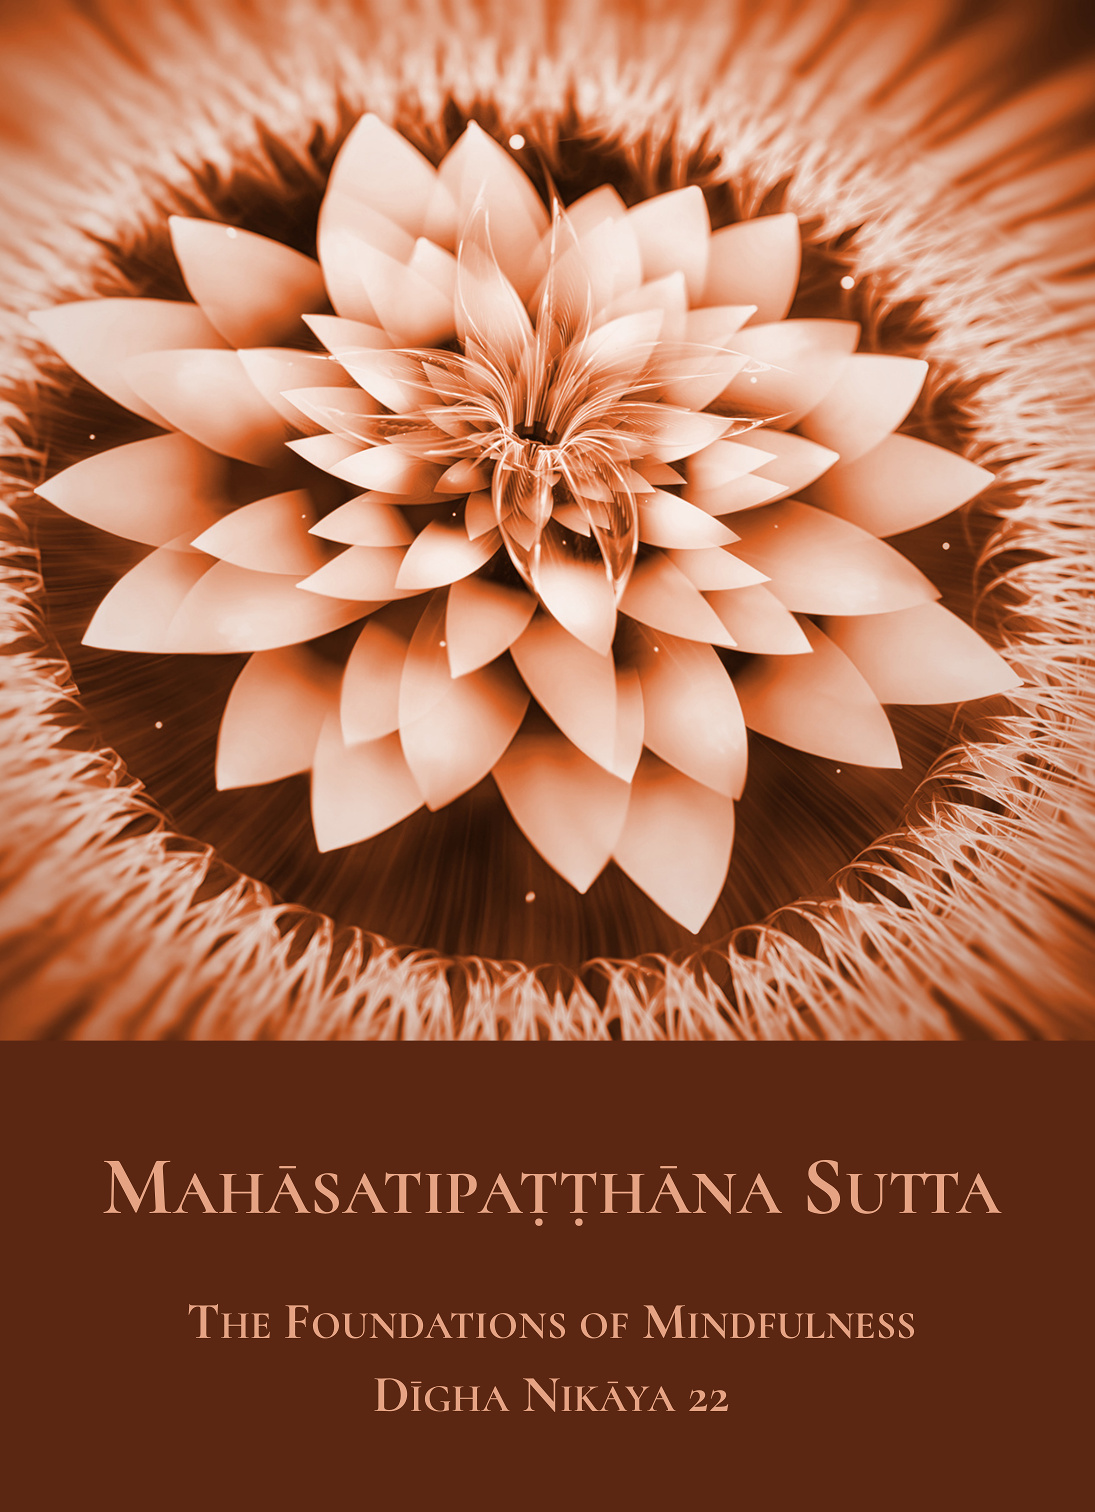
\includegraphics[height=\paperheight]{satipatthana-webcover.jpg}%
}

\cleartoverso
\thispagestyle{empty}\mbox{}

\addtocontents{toc}{\protect \enlargethispage {2\baselineskip}}

\cleartorecto
\tableofcontents*

\clearpage
\thispagestyle{empty}

{\fontsize{9}{12}\selectfont
\mbox{}

\vfill

Pali text from the Mahāsaṅgīti Tipiṭaka Buddhavasse 2500: World Tipiṭaka Edition
in Roman Script. Edited and published by The M.L. Maniratana Bunnag Dhamma
Society Fund, 2005. Based on the digital edition of the Chaṭṭha Saṅgāyana
published by the Vipassana Research Institute, with corrections and proofreading
by the Dhamma Society.

https://suttacentral.net/dn22/pli/ms

}

\mainmatter

\showpartnumberfalse
\cleartorecto
\thispagestyle{empty}
\markboth{\leftmark}{Mahāsatipaṭṭhāna Sutta}

\printparttitle{%
Mahāsatipaṭṭhāna Sutta

\vspace*{2em}

{\sectionFont\sectionSize\color{section}%
  The Foundations of Mindfulness

  \bigskip

  Dīgha Nikāya 22
\par}

}

\artopttrue

\newcommand\englishPage{%
  \clearpage%
  \englishText%
  %\markboth{\englishTitle}{\rightmark}%
}

\newcommand\paliPage{%
  \clearpage%
  \paliText%
  %\markboth{\paliTitle}{\rightmark}%
}

\renewcommand{\englishTitle}{The Foundations of Mindfulness}
\renewcommand{\paliTitle}{Mahāsatipaṭṭhāna Sutta}

\englishPage
\chapter{Introduction}

Thus have I heard.

On one occasion the Blessed One was in the Kuru country where there was a town
of the Kurus named Kammāsadhamma. There the Blessed One addressed the bhikkhus
thus: “Bhikkhus.” “Bhante,” the bhikkhus replied to the Blessed One. The Blessed
One said this:

“Bhikkhus, this is the one-way path for the purification of beings, for the
surmounting of sorrow and lamentation, for the passing away of pain and
dejection, for the attainment of the true way, for the realisation of Nibbāna,
namely, the four foundations of mindfulness. What are the four?

Here, bhikkhus, a bhikkhu dwells contemplating the body in the body, ardent,
clearly comprehending, and mindful, having subdued longing and dejection in
regard to the world. He dwells contemplating feelings in feelings, ardent,
clearly comprehending, and mindful, having subdued longing and dejection in
regard to the world. He dwells contemplating mind in mind, ardent, clearly
comprehending, and mindful, having subdued longing and dejection in regard to
the world. He dwells contemplating phenomena in phenomena, ardent, clearly
comprehending, and mindful, having subdued longing and dejection in regard to
the world.

\instr{The Introduction is finished.}

\paliPage
\chapter*{Uddeso}

[Evaṁ me sutaṁ]

Ekaṁ samayaṁ bhagavā kurūsu viharati kammāsadhammaṁ nāma kurūnaṁ nigamo. Tatra
kho꜔꜒ bhagavā bhikkhū꜔꜒ āmantesi: “bhikkhavo”ti. “Bhaddante”ti te bhikkhū꜔꜒ bhagavato
paccasso꜔꜒su꜔꜒ṁ. Bhagavā etadavoca:

“Ekāyano ayaṁ, bhikkhave, maggo sattānaṁ visuddhiyā, so꜔꜒ka-paridevānaṁ
samatikkamāya dukkha-domanassā꜔꜒naṁ attha꜔꜒ṅgamāya ñāyassa adhigamāya nibbānassa
sacchikiriyāya, yadidaṁ cattāro satipaṭṭhā꜔꜒nā.

Katame cattāro? Idha, bhikkhave, bhikkhu kāye kāyānupassī꜔꜒ viharati ātāpī
sa꜔꜒mpajāno satimā vineyya loke abhijjhā-domanassa꜔꜒ṁ, vedanāsu vedanānupassī꜔꜒
viharati ātāpī sa꜔꜒mpajāno satimā vineyya loke abhijjhā-domanassa꜔꜒ṁ, citte
cittānupassī꜔꜒ viharati ātāpī sa꜔꜒mpajāno satimā vineyya loke abhijjhā-domanassa꜔꜒ṁ,
dhammesu dhammānupassī꜔꜒ viharati ātāpī sa꜔꜒mpajāno satimā vineyya loke
abhijjhā-domanassa꜔꜒ṁ.

\instr{Uddeso niṭṭhito.}

\englishPage
\chapter{Contemplation of the Body}

\section{Mindfulness of Breathing}

And how, bhikkhus, does a bhikkhu dwell contemplating\\
the body in the body?

Here, bhikkhus, a bhikkhu, gone to the forest, to the foot of a tree, or to an
empty hut, sits down; having folded his legs crosswise, straightened his body,
and established mindfulness in front of him.

Just mindful he breathes in, mindful he breathes out.\\
Breathing in long, he understands: ‘I breathe in long’;\\
or breathing out long, he understands: ‘I breathe out long.’\\
Breathing in short, he understands: ‘I breathe in short’;\\
or breathing out short, he understands: ‘I breathe out short.’\\
He trains thus: ‘I will breathe in experiencing the whole body’;\\
he trains thus:‘I will breathe out experiencing the whole body.’\\
He trains thus: ‘I will breathe in tranquilising the bodily formation’;\\
he trains thus: ‘I will breathe out tranquilising the bodily formation.’

Just as, bhikkhus, a skilled lathe-worker or his apprentice,\\
when making a long turn, understands: ‘I make a long turn’;\\
or, when making a short turn, understands: ‘I make a short turn’;\\
so too, bhikkhus, a bhikkhu\\
breathing in long, he understands: ‘I breathe in long’;\\
or breathing out long, he understands: ‘I breathe out long.’\\
Breathing in short, he understands: ‘I breathe in short’;\\
or breathing out short, he understands: ‘I breathe out short.’\\
He trains thus: ‘I will breathe in experiencing the whole body’;\\
he trains thus: ‘I will breathe out experiencing the whole body.’\\
He trains thus: ‘I will breathe in tranquilising the bodily formation’;\\
he trains thus: ‘I will breathe out tranquilising the bodily formation.’

\paliPage
\chapter*{Kāyānupassanā}

\section*{Ānāpānapabbaṁ}

Katha꜔꜒ñca pana, bhikkhave, bhikkhu kāye kāyānupassī꜔꜒ viharati?

Idha, bhikkhave, bhikkhu araññagato vā rukkhamūlagato vā su꜔꜒ññāgāragato vā
nisī꜔꜒dati pallaṅkaṁ ābhujitvā ujuṁ kāyaṁ paṇidhāya parimukha꜔꜒ṁ satiṁ upaṭṭhapetvā.
so꜔꜒ satova assasati, satova passasati.

Dīghaṁ vā assasa꜔꜒nto ‘dīghaṁ assasā꜔꜒mī’ti pajānāti,\\
dīghaṁ vā passasa꜔꜒nto ‘dīghaṁ passasā꜔꜒mī’ti pajānāti.\\
rassa꜔꜒ṁ vā assasa꜔꜒nto ‘rassa꜔꜒ṁ assasā꜔꜒mī’ti pajānāti,\\
rassa꜔꜒ṁ vā passasa꜔꜒nto ‘rassa꜔꜒ṁ passasā꜔꜒mī’ti pajānāti.\\
‘sabbakāya-paṭisa꜔꜒ṁvedī assasissā꜔꜒mī’ti sikkhati,\\
‘sabbakāya-paṭisa꜔꜒ṁvedī passasissā꜔꜒mī’ti sikkhati.\\
‘passa꜔꜒mbhayaṁ kāyasa꜔꜒ṅkhā꜔꜒raṁ assasissā꜔꜒mī’ti sikkhati,\\
‘passa꜔꜒mbhayaṁ kāyasa꜔꜒ṅkhā꜔꜒raṁ passasissā꜔꜒mī’ti sikkhati.

Se꜔꜒yyathā꜔꜒pi, bhikkhave, dakkho꜔꜒ bhamakāro vā bhamakārantevāsī꜔꜒ vā\\
dīghaṁ vā añcha꜔꜒nto ‘dīghaṁ añchā꜔꜒mī’ti pajānāti,\\
rassa꜔꜒ṁ vā añcha꜔꜒nto ‘rassa꜔꜒ṁ añchā꜔꜒mī’ti pajānāti;\\
evameva kho꜔꜒, bhikkhave, bhikkhu\\
dīghaṁ vā assasa꜔꜒nto ‘dīghaṁ assasā꜔꜒mī’ti pajānāti,\\
dīghaṁ vā passasa꜔꜒nto ‘dīghaṁ passasā꜔꜒mī’ti pajānāti,\\
rassa꜔꜒ṁ vā assasa꜔꜒nto ‘rassa꜔꜒ṁ assasā꜔꜒mī’ti pajānāti,\\
rassa꜔꜒ṁ vā passasa꜔꜒nto ‘rassa꜔꜒ṁ passasā꜔꜒mī’ti pajānāti.\\
‘sabbakāya-paṭisa꜔꜒ṁvedī assasissā꜔꜒mī’ti sikkhati,\\
‘sabbakāya-paṭisa꜔꜒ṁvedī passasissā꜔꜒mī’ti sikkhati,\\
‘passa꜔꜒mbhayaṁ kāyasa꜔꜒ṅkhā꜔꜒raṁ assasissā꜔꜒mī’ti sikkhati,\\
‘passa꜔꜒mbhayaṁ kāyasa꜔꜒ṅkhā꜔꜒raṁ passasissā꜔꜒mī’ti sikkhati.

\englishPage

In this way he dwells contemplating the body in the body internally, or he
dwells contemplating the body in the body externally, or he dwells contemplating
the body in the body both internally and externally. Or else he dwells
contemplating in the body its nature of arising, or he dwells contemplating in
the body its nature of vanishing, or he dwells contemplating in the body its
nature of both arising and vanishing. Or else mindfulness that ‘there is a body’
is simply established in him to the extent necessary for bare knowledge and
repeated mindfulness.

And he dwells independent, not clinging to anything in the world. That is how,
bhikkhus, a bhikkhu dwells contemplating the body in the body.

\instr{The section on Mindfulness of Breathing is finished.}

\section{The Four Postures}

Again, bhikkhus, a bhikkhu when walking, understands: ‘I am walking’; when
standing, he understands: ‘I am standing’; when sitting, he understands: ‘I am
sitting’; when lying down, he understands: ‘I am lying down’; or however his
body is disposed, he understands it accordingly.

In this way he dwells contemplating the body in the body internally, or he
dwells contemplating the body in the body externally, or he dwells contemplating
the body in the body both internally and externally. Or else he dwells
contemplating in the body its nature of arising, or he dwells contemplating in
the body its nature of vanishing, or he dwells contemplating in the body its
nature of both arising and vanishing. Or else mindfulness that ‘there is a body’
is simply established in him to the extent necessary for bare knowledge and
repeated mindfulness.

And he dwells independent, not clinging to anything in the world. That is how,
bhikkhus, a bhikkhu dwells contemplating the body in the body.

\instr{The section on the Four Postures is finished.}

\paliPage

Iti ajjhattaṁ vā kāye kāyānupassī꜔꜒ viharati, bahiddhā vā kāye kāyānupassī꜔꜒
viharati, ajjhatta-bahiddhā vā kāye kāyānupassī꜔꜒ viharati. samudaya-dhammānupassī꜔꜒
vā kāyasmi꜔꜒ṁ viharati, vaya-dhammā-\\
nupassī꜔꜒ vā kāyasmi꜔꜒ṁ viharati, samudaya-vaya-dhammānupassī꜔꜒ vā kāyasmi꜔꜒ṁ viharati.
‘atthi kāyo’ti vā panassa sati paccupaṭṭhitā ho꜔꜒ti yāvadeva ñāṇamattāya
paṭissatimattāya anissito ca viharati, na ca kiñci loke upādiyati. evampi kho꜔꜒,
bhikkhave, bhikkhu kāye kāyānupassī꜔꜒ viharati.

\instr{Ānāpānapabbaṁ niṭṭhitaṁ.}

\section*{Iriyāpathapabba}

Puna caparaṁ, bhikkhave, bhikkhu gaccha꜔꜒nto vā ‘gacchā꜔꜒mī’ti pajānāti, ṭhito vā
‘ṭhitomhī꜔꜒’ti pajānāti, nisi꜔꜒nno vā ‘nisi꜔꜒nnomhī꜔꜒’ti pajānāti, sayāno vā
‘sayānomhī꜔꜒’ti pajānāti, yathā꜔꜒ yathā꜔꜒ vā panassa kāyo paṇihito ho꜔꜒ti tathā꜔꜒ tathā꜔꜒
naṁ pajānāti.

Iti ajjhattaṁ vā kāye kāyānupassī꜔꜒ viharati, bahiddhā vā kāye kāyānupassī꜔꜒
viharati, ajjhatta-bahiddhā vā kāye kāyānupassī꜔꜒ viharati. samudaya-dhammānupassī꜔꜒
vā kāyasmi꜔꜒ṁ viharati, vaya-dhammā-\\
nupassī꜔꜒ vā kāyasmi꜔꜒ṁ viharati, samudaya-vaya-dhammānupassī꜔꜒ vā kāyasmi꜔꜒ṁ viharati.
‘atthi kāyo’ti vā panassa sati paccupaṭṭhitā ho꜔꜒ti yāvadeva ñāṇamattāya
paṭissatimattāya anissito ca viharati, na ca kiñci loke upādiyati. evampi kho꜔꜒,
bhikkhave, bhikkhu kāye kāyānupassī꜔꜒ viharati.

\instr{Iriyāpathapabbaṁ niṭṭhitaṁ.}

\englishPage
\section{Clear Comprehension}

Again, bhikkhus, a bhikkhu is one who acts with clear comprehension when going
forward and returning, who acts with clear comprehension when looking ahead and
looking away; who acts with clear comprehension when bending and stretching his
limbs; who acts with clear comprehension when wearing his robes and carrying his
outer robe and bowl; who acts with clear comprehension when eating, drinking,
chewing, and tasting; who acts with clear comprehension when defecating and
urinating; who acts with clear comprehension when walking, standing, sitting,
falling asleep, waking up, talking and keeping silent.

In this way he dwells contemplating the body in the body internally, or he
dwells contemplating the body in the body externally, or he dwells contemplating
the body in the body both internally and externally. Or else he dwells
contemplating in the body its nature of arising, or he dwells contemplating in
the body its nature of vanishing, or he dwells contemplating in the body its
nature of both arising and vanishing. Or else mindfulness that ‘there is a body’
is simply established in him to the extent necessary for bare knowledge and
repeated mindfulness.

And he dwells independent, not clinging to anything in the world. That is how,
bhikkhus, a bhikkhu dwells contemplating the body in the body.

\instr{The section on Clear Comprehension is finished.}

\section{Unattractiveness of the Body}

Again, bhikkhus, a bhikkhu reviews this same body up from the soles of the feet
and down from the top of the hair, bounded by skin, as full of many kinds of
impurity thus:

\enlargethispage{2\baselineskip}

‘In this body there are head-hairs, body hairs, nails, teeth, skin, flesh,
sinews, bones, bone-marrow, kidneys, heart, liver, diaphragm, spleen, lungs,
intestines, mesentery, stomach, feces, bile, phlegm, pus, blood, sweat, fat,
tears, grease, spittle, snot, oil of the joints, and urine.’

\paliPage
\section*{Sampajānapabba}

Puna caparaṁ, bhikkhave, bhikkhu abhikkante paṭikkante sa꜔꜒mpajānakārī ho꜔꜒ti,
ālokite vilokite sa꜔꜒mpajānakārī ho꜔꜒ti, samiñjite pasā꜔꜒rite sa꜔꜒mpajānakārī ho꜔꜒ti,
sa꜔꜒ṅghāṭi-patta-cīvara-dhāraṇe sa꜔꜒mpajānakārī ho꜔꜒ti, asite pīte khā꜔꜒yite sā꜔꜒yite
sa꜔꜒mpajānakārī ho꜔꜒ti, uccāra-passā꜔꜒va-kamme sa꜔꜒mpajānakārī ho꜔꜒ti, gate ṭhite nisi꜔꜒nne
sutte jāgarite bhāsite tuṇhī꜔꜒bhāve sa꜔꜒mpajānakārī ho꜔꜒ti.

Iti ajjhattaṁ vā kāye kāyānupassī꜔꜒ viharati, bahiddhā vā kāye kāyānupassī꜔꜒
viharati, ajjhatta-bahiddhā vā kāye kāyānupassī꜔꜒ viharati. samudaya-dhammānupassī꜔꜒
vā kāyasmi꜔꜒ṁ viharati, vaya-dhammā-\\
nupassī꜔꜒ vā kāyasmi꜔꜒ṁ viharati, samudaya-vaya-dhammānupassī꜔꜒ vā kāyasmi꜔꜒ṁ viharati.
‘atthi kāyo’ti vā panassa sati paccupaṭṭhitā ho꜔꜒ti yāvadeva ñāṇamattāya
paṭissatimattāya anissito ca viharati, na ca kiñci loke upādiyati. evampi kho꜔꜒,
bhikkhave, bhikkhu kāye kāyānupassī꜔꜒ viharati.

\instr{Sampajānapabbaṁ niṭṭhitaṁ.}

\section*{Paṭikūla-manasikārapabba}

Puna caparaṁ, bhikkhave, bhikkhu imameva kāyaṁ uddhaṁ pādatalā adho kesamatthakā
tacapariyantaṁ pūraṁ nānappakārassa asucino paccavekkhati:

‘Atthi imasmi꜔꜒ṁ kāye kesā꜔꜒ lomā nakhā꜔꜒ dantā taco, maṁsa꜔꜒ṁ nahā꜔꜒rū aṭṭhī꜔꜒ aṭṭhimiñjaṁ
vakkaṁ, hadayaṁ yakanaṁ kilomakaṁ pihakaṁ papphā꜔꜒sa꜔꜒ṁ, antaṁ antaguṇaṁ udariyaṁ
karīsa꜔꜒ṁ, pittaṁ se꜔꜒mha꜔꜒ṁ pubbo lohitaṁ se꜔꜒do medo, assu vasā꜔꜒ khe꜔꜒ḷo si꜔꜒ṅghāṇikā
lasikā muttan’ti.

\englishPage

Just as though, bhikkhus, there were a bag with an opening at both ends full of
many sorts of grain, such as hill rice, red rice, beans, peas, millet, and white
rice, and a man with good eyes were to open it and review it thus:

‘This is hill rice, this is red rice, these are beans, these are peas, this is
millet, this is white rice’; so too, bhikkhus, a bhikkhu reviews this same body
up from the soles of the feet and down from the top of the hair, bounded by
skin, as full of many kinds of impurity thus:

'In this body there are head-hairs, body hairs, nails, teeth, skin, flesh,
sinews, bones, bone-marrow, kidneys, heart, liver, diaphragm, spleen, lungs,
intestines, mesentery, stomach, feces, bile, phlegm, pus, blood, sweat, fat,
tears, grease, spittle, snot, oil of the joints, and urine.'

In this way he dwells contemplating the body in the body internally, or he
dwells contemplating the body in the body externally, or he dwells contemplating
the body in the body both internally and externally. Or else he dwells
contemplating in the body its nature of arising, or he dwells contemplating in
the body its nature of vanishing, or he dwells contemplating in the body its
nature of both arising and vanishing. Or else mindfulness that ‘there is a body’
is simply established in him to the extent necessary for bare knowledge and
repeated mindfulness.

And he dwells independent, not clinging to anything in the world. That is how,
bhikkhus, a bhikkhu dwells contemplating the body in the body.

\instr{The section on Unattractiveness of the Body is finished.}

\paliPage

Se꜔꜒yyathā꜔꜒pi, bhikkhave, ubhatomukhā꜔꜒ putoḷi pūrā nānāvihitassa dhaññassa,
se꜔꜒yyathī꜔꜒daṁ, sā꜔꜒līnaṁ vīhī꜔꜒naṁ muggānaṁ māsā꜔꜒naṁ tilānaṁ taṇḍulānaṁ. Tamenaṁ
cakkhumā puriso꜔꜒ muñcitvā paccavekkhe꜔꜒yya:

‘Ime sā꜔꜒lī, ime vīhī꜔꜒ ime muggā ime māsā꜔꜒ ime tilā ime taṇḍulā’ti. Evameva kho꜔꜒,
bhikkhave, bhikkhu imameva kāyaṁ uddhaṁ pādatalā adho kesamatthakā
tacapariyantaṁ pūraṁ nānappakārassa asucino paccavekkhati:

‘Atthi imasmi꜔꜒ṁ kāye kesā꜔꜒ lomā nakhā꜔꜒ dantā taco, maṁsa꜔꜒ṁ nahā꜔꜒rū aṭṭhī꜔꜒ aṭṭhimiñjaṁ
vakkaṁ, hadayaṁ yakanaṁ kilomakaṁ pihakaṁ papphā꜔꜒sa꜔꜒ṁ, antaṁ antaguṇaṁ udariyaṁ
karīsa꜔꜒ṁ, pittaṁ se꜔꜒mha꜔꜒ṁ pubbo lohitaṁ se꜔꜒do medo, assu vasā꜔꜒ khe꜔꜒ḷo si꜔꜒ṅghāṇikā
lasikā muttan’ti.

Iti ajjhattaṁ vā kāye kāyānupassī꜔꜒ viharati, bahiddhā vā kāye kāyānupassī꜔꜒
viharati, ajjhatta-bahiddhā vā kāye kāyānupassī꜔꜒ viharati. samudaya-dhammānupassī꜔꜒
vā kāyasmi꜔꜒ṁ viharati, vaya-dhammā-\\
nupassī꜔꜒ vā kāyasmi꜔꜒ṁ viharati, samudaya-vaya-dhammānupassī꜔꜒ vā kāyasmi꜔꜒ṁ viharati.
‘atthi kāyo’ti vā panassa sati paccupaṭṭhitā ho꜔꜒ti yāvadeva ñāṇamattāya
paṭissatimattāya anissito ca viharati, na ca kiñci loke upādiyati. evampi kho꜔꜒,
bhikkhave, bhikkhu kāye kāyānupassī꜔꜒ viharati.

\instr{Paṭikūla-manasikārapabbaṁ niṭṭhitaṁ.}

\englishPage
\section{Elements}

Again, bhikkhus, a bhikkhu reviews this same body, however it is placed, however
disposed, as consisting of elements thus: `In this body there are the earth
element, the water element, the fire element, and the air element.'

Just as though, bhikkhus, a skilled butcher or his apprentice had killed a cow
and were seated at the crossroads with it cut up into pieces; so too, bhikkhus,
a bhikkhu reviews this same body, however it is placed, however disposed, as
consisting of elements thus: `In this body there are the earth element, the
water element, the fire element, and the air element.'

In this way he dwells contemplating the body in the body internally, or he
dwells contemplating the body in the body externally, or he dwells contemplating
the body in the body both internally and externally. Or else he dwells
contemplating in the body its nature of arising, or he dwells contemplating in
the body its nature of vanishing, or he dwells contemplating in the body its
nature of both arising and vanishing. Or else mindfulness that ‘there is a body’
is simply established in him to the extent necessary for bare knowledge and
repeated mindfulness.

And he dwells independent, not clinging to anything in the world. That is how,
bhikkhus, a bhikkhu dwells contemplating the body in the body.

\instr{The section on Elements is finished.}

\section{Nine Charnel Ground Contemplations}

[1] Again, bhikkhus, as though he were to see a corpse thrown aside in a charnel
ground, one, two, or three days dead, bloated, livid, and oozing matter, a
bhikkhu compares this same body with it thus: 'This body too is of the same
nature, it will be like that, it is not exempt from that fate.'

\paliPage
\section*{Dhātu-manasikārapabba}

Puna caparaṁ, bhikkhave, bhikkhu imameva kāyaṁ yathā꜔꜒ṭhitaṁ yathā꜔꜒paṇihitaṁ
dhātuso꜔꜒ paccavekkhati: ‘atthi imasmi꜔꜒ṁ kāye pathavīdhātu āpodhātu tejodhātu
vāyodhātū’ti.

Se꜔꜒yyathā꜔꜒pi, bhikkhave, dakkho꜔꜒ goghātako vā goghātakantevāsī꜔꜒ vā gāviṁ vadhitvā
cātummahā꜔꜒pathe꜔꜒ bilaso꜔꜒ vibhajitvā nisi꜔꜒nno assa; evameva kho꜔꜒, bhikkhave, bhikkhu
imameva kāyaṁ yathā꜔꜒ṭhitaṁ yathā꜔꜒paṇihitaṁ dhātuso꜔꜒ paccavekkhati: ‘atthi imasmi꜔꜒ṁ
kāye pathavīdhātu āpodhātu tejodhātu vāyodhātū’ti.

Iti ajjhattaṁ vā kāye kāyānupassī꜔꜒ viharati, bahiddhā vā kāye kāyānupassī꜔꜒
viharati, ajjhatta-bahiddhā vā kāye kāyānupassī꜔꜒ viharati. samudaya-dhammānupassī꜔꜒
vā kāyasmi꜔꜒ṁ viharati, vaya-dhammā-\\
nupassī꜔꜒ vā kāyasmi꜔꜒ṁ viharati, samudaya-vaya-dhammānupassī꜔꜒ vā kāyasmi꜔꜒ṁ viharati.
‘atthi kāyo’ti vā panassa sati paccupaṭṭhitā ho꜔꜒ti yāvadeva ñāṇamattāya
paṭissatimattāya anissito ca viharati, na ca kiñci loke upādiyati. evampi kho꜔꜒,
bhikkhave, bhikkhu kāye kāyānupassī꜔꜒ viharati.

\instr{Dhātu-manasikārapabbaṁ niṭṭhitaṁ.}

\section*{Navasivathikapabba}

[1] Puna caparaṁ, bhikkhave, bhikkhu se꜔꜒yyathā꜔꜒pi passe꜔꜒yya sarīraṁ sivathikāya
chaḍḍitaṁ ekāhamataṁ vā dvīhamataṁ vā tīhamataṁ vā uddhumātakaṁ vinīlakaṁ
vipubbakajātaṁ. So꜔꜒ imameva kāyaṁ upasa꜔꜒ṁharati: ‘ayampi kho꜔꜒ kāyo evaṁ-dhammo
evaṁ-bhāvī evaṁ-anatīto’ti.

\englishPage

In this way he dwells contemplating the body in the body internally, or he
dwells contemplating the body in the body externally, or he dwells contemplating
the body in the body both internally and externally. Or else he dwells
contemplating in the body its nature of arising, or he dwells contemplating in
the body its nature of vanishing, or he dwells contemplating in the body its
nature of both arising and vanishing. Or else mindfulness that ‘there is a body’
is simply established in him to the extent necessary for bare knowledge and
repeated mindfulness.

And he dwells independent, not clinging to anything in the world. That is how,
bhikkhus, a bhikkhu dwells contemplating the body in the body.

[2] Again, bhikkhus, as though he were to see a corpse thrown aside in a charnel
ground, being devoured by crows, being devoured by vultures, being devoured by
hawks, being devoured by dogs, being devoured by jackals, or being devoured by
various kinds of worms, a bhikkhu compares this same body with it thus: 'This
body too is of the same nature, it will be like that, it is not exempt from that
fate.'

In this way he dwells contemplating the body in the body internally, or he
dwells contemplating the body in the body externally, or he dwells contemplating
the body in the body both internally and externally. Or else he dwells
contemplating in the body its nature of arising, or he dwells contemplating in
the body its nature of vanishing, or he dwells contemplating in the body its
nature of both arising and vanishing. Or else mindfulness that ‘there is a body’
is simply established in him to the extent necessary for bare knowledge and
repeated mindfulness.

And he dwells independent, not clinging to anything in the world. That is how,
bhikkhus, a bhikkhu dwells contemplating the body in the body.

\paliPage

Iti ajjhattaṁ vā kāye kāyānupassī꜔꜒ viharati, bahiddhā vā kāye kāyānupassī꜔꜒
viharati, ajjhatta-bahiddhā vā kāye kāyānupassī꜔꜒ viharati. samudaya-dhammānupassī꜔꜒
vā kāyasmi꜔꜒ṁ viharati, vaya-dhammā-\\
nupassī꜔꜒ vā kāyasmi꜔꜒ṁ viharati, samudaya-vaya-dhammānupassī꜔꜒ vā kāyasmi꜔꜒ṁ viharati.
‘atthi kāyo’ti vā panassa sati paccupaṭṭhitā ho꜔꜒ti yāvadeva ñāṇamattāya
paṭissatimattāya anissito ca viharati, na ca kiñci loke upādiyati. evampi kho꜔꜒,
bhikkhave, bhikkhu kāye kāyānupassī꜔꜒ viharati.

[2] Puna caparaṁ, bhikkhave, bhikkhu se꜔꜒yyathā꜔꜒pi passe꜔꜒yya sarīraṁ sivathikāya
chaḍḍitaṁ kākehi vā khajjamānaṁ kulalehi vā khajjamānaṁ gijjhehi vā khajjamānaṁ
kaṅkehi vā khajjamānaṁ sunakhe꜔꜒hi vā khajjamānaṁ byagghehi vā khajjamānaṁ dīpīhi
vā khajjamānaṁ si꜔꜒ṅgālehi vā khajjamānaṁ vividhehi vā pāṇakajātehi khajjamānaṁ.
So꜔꜒ imameva kāyaṁ upasa꜔꜒ṁharati: ‘ayampi kho꜔꜒ kāyo evaṁ-dhammo evaṁ-bhāvī
evaṁ-anatīto’ti.

Iti ajjhattaṁ vā kāye kāyānupassī꜔꜒ viharati, bahiddhā vā kāye kāyānupassī꜔꜒
viharati, ajjhatta-bahiddhā vā kāye kāyānupassī꜔꜒ viharati. samudaya-dhammānupassī꜔꜒
vā kāyasmi꜔꜒ṁ viharati, vaya-dhammā-\\
nupassī꜔꜒ vā kāyasmi꜔꜒ṁ viharati, samudaya-vaya-dhammānupassī꜔꜒ vā kāyasmi꜔꜒ṁ viharati.
‘atthi kāyo’ti vā panassa sati paccupaṭṭhitā ho꜔꜒ti yāvadeva ñāṇamattāya
paṭissatimattāya anissito ca viharati, na ca kiñci loke upādiyati. evampi kho꜔꜒,
bhikkhave, bhikkhu kāye kāyānupassī꜔꜒ viharati.

\englishPage

[3]~Again, bhikkhus, as though he were to see a corpse thrown aside in a
charnel ground, a skeleton with flesh and blood, held together with sinews~\ldots{}

[4]~a fleshless skeleton smeared with blood, held together with sinews~\ldots{}

[5]~a skeleton without flesh and blood, held together with sinews~\ldots{}

[6]~disconnected bones not held together with sinews scattered in all directions
-- here a hand-bone, there a foot bone, here a shin-bone, there a thigh-bone,
here a hip-bone, there a back-bone, here a rib-bone, there a chest-bone, here an
arm-bone, there a shoulder-bone, here a neck-bone, there a jaw-bone, here a
tooth-bone, there the skull -- a bhikkhu compares this same body with it thus:
`This body too is of the same nature, it will be like that, it is not exempt
from that fate.'

In this way he dwells contemplating the body in the body internally, or he
dwells contemplating the body in the body externally, or he dwells contemplating
the body in the body both internally and externally. Or else he dwells
contemplating in the body its nature of arising, or he dwells contemplating in
the body its nature of vanishing, or he dwells contemplating in the body its
nature of both arising and vanishing. Or else mindfulness that ‘there is a body’
is simply established in him to the extent necessary for bare knowledge and
repeated mindfulness.

And he dwells independent, not clinging to anything in the world. That is how,
bhikkhus, a bhikkhu dwells contemplating the body in the body.

[7] Again, bhikkhus, as though he were to see a corpse thrown aside in a charnel
ground, bones bleached white, the colour of shells~\ldots{}

[8]~bones heaped up, more than a year old~\ldots{}

\paliPage

[3]~Puna caparaṁ, bhikkhave, bhikkhu se꜔꜒yyathā꜔꜒pi passe꜔꜒yya sarīraṁ sivathikāya
chaḍḍitaṁ aṭṭhika-sa꜔꜒ṅkhalikaṁ samaṁsa-lohitaṁ nahā꜔꜒ru-sa꜔꜒mbandhaṁ~\ldots{}

[4]~Aṭṭhika-sa꜔꜒ṅkhalikaṁ nimaṁsa-lohita-makkhitaṁ nahā꜔꜒ru-sa꜔꜒mbandhaṁ~\ldots{}

[5]~Aṭṭhika-sa꜔꜒ṅkhalikaṁ apagata-maṁsa-lohitaṁ nahā꜔꜒ru-sa꜔꜒mbandhaṁ~\ldots{}

[6]~Aṭṭhikāni apagata-sa꜔꜒mbandhāni disā꜔꜒ vidisā꜔꜒ vikkhittāni, aññena hatth'aṭṭhikaṁ
aññena pād'aṭṭhikaṁ aññena gopphak'aṭṭhikaṁ aññena jaṅgh'aṭṭhikaṁ aññena ūr'uṭṭhikaṁ
aññena kaṭ'iṭṭhikaṁ aññena phā꜔꜒suk'aṭṭhikaṁ aññena piṭṭh'iṭṭhikaṁ aññena
kha꜔꜒ndh'aṭṭhikaṁ aññena gīv'aṭṭhikaṁ aññena hanuk'aṭṭhikaṁ aññena dant'aṭṭhikaṁ
aññena sī꜔꜒sakaṭāha꜔꜒ṁ. So꜔꜒ imameva kāyaṁ upasa꜔꜒ṁharati: ‘ayampi kho꜔꜒ kāyo evaṁdhammo
evaṁbhāvī evaṁanatīto’ti.

Iti ajjhattaṁ vā kāye kāyānupassī꜔꜒ viharati, bahiddhā vā kāye kāyānupassī꜔꜒
viharati, ajjhatta-bahiddhā vā kāye kāyānupassī꜔꜒ viharati. samudaya-dhammānupassī꜔꜒
vā kāyasmi꜔꜒ṁ viharati, vaya-dhammā-\\
nupassī꜔꜒ vā kāyasmi꜔꜒ṁ viharati, samudaya-vaya-dhammānupassī꜔꜒ vā kāyasmi꜔꜒ṁ viharati.
‘atthi kāyo’ti vā panassa sati paccupaṭṭhitā ho꜔꜒ti yāvadeva ñāṇamattāya
paṭissatimattāya anissito ca viharati, na ca kiñci loke upādiyati. evampi kho꜔꜒,
bhikkhave, bhikkhu kāye kāyānupassī꜔꜒ viharati.

[7]~Puna caparaṁ, bhikkhave, bhikkhu se꜔꜒yyathā꜔꜒pi passe꜔꜒yya sarīraṁ sivathikāya
chaḍḍitaṁ aṭṭhikāni se꜔꜒tāni sa꜔꜒ṅkha-vaṇṇa-paṭibhāgāni~\ldots{}

[8]~Aṭṭhikāni puñjakitāni terovassikāni~\ldots{}

\englishPage

[9]~bones rotted and crumbled to dust, a bhikkhu compares this same
body with it thus: ‘This body too is of the same nature, it will be like that,
it is not exempt from that fate.’

In this way he dwells contemplating the body in the body internally, or he
dwells contemplating the body in the body externally, or he dwells contemplating
the body in the body both internally and externally. Or else he dwells
contemplating in the body its nature of arising, or he dwells contemplating in
the body its nature of vanishing, or he dwells contemplating in the body its
nature of both arising and vanishing. Or else mindfulness that ‘there is a body’
is simply established in him to the extent necessary for bare knowledge and
repeated mindfulness.

And he dwells independent, not clinging to anything in the world. That is how,
bhikkhus, a bhikkhu dwells contemplating the body in the body.

\instr{The section on the Nine Charnel Ground Contemplations is finished.}

\instr{Contemplation of the Body is finished.}

\paliPage

[9]~Aṭṭhikāni pūtīni cuṇṇakajātāni. so꜔꜒ imameva kāyaṁ upasa꜔꜒ṁharati: ‘ayampi kho꜔꜒
kāyo evaṁ-dhammo evaṁ-bhāvī evaṁ-anatīto’ti.

Iti ajjhattaṁ vā kāye kāyānupassī꜔꜒ viharati, bahiddhā vā kāye kāyānupassī꜔꜒
viharati, ajjhatta-bahiddhā vā kāye kāyānupassī꜔꜒ viharati. samudaya-dhammānupassī꜔꜒
vā kāyasmi꜔꜒ṁ viharati, vaya-dhammā-\\
nupassī꜔꜒ vā kāyasmi꜔꜒ṁ viharati, samudaya-vaya-dhammānupassī꜔꜒ vā kāyasmi꜔꜒ṁ viharati.
‘atthi kāyo’ti vā panassa sati paccupaṭṭhitā ho꜔꜒ti yāvadeva ñāṇamattāya
paṭissatimattāya anissito ca viharati, na ca kiñci loke upādiyati. evampi kho꜔꜒,
bhikkhave, bhikkhu kāye kāyānupassī꜔꜒ viharati.

\instr{Navasivathikapabbaṁ niṭṭhitaṁ.}

\instr{Kāyānupassanā niṭṭhitā.}

\englishPage
\chapter{Contemplation of Feelings}

And how, bhikkhus, does a bhikkhu dwell contemplating feelings in feelings?

Here, bhikkhus, when feeling a pleasant feeling, a bhikkhu understands:
`I~feel a pleasant feeling';
when feeling a painful feeling, he understands:
`I~feel a painful feeling';
when feeling a neither-painful-nor-pleasant feeling, he understands:
`I~feel a neither-painful-nor-pleasant feeling.'

When feeling a carnal pleasant feeling, he understands:
`I~feel a carnal pleasant feeling';
when feeling a spiritual pleasant feeling, he understands:
`I~feel a spiritual pleasant feeling';
when feeling a carnal painful feeling, he understands:
`I~feel a carnal painful feeling';
when feeling a spiritual painful feeling, he understands:
`I~feel a spiritual painful feeling';
when feeling a carnal neither-painful-nor-pleasant feeling, he understands:
`I~feel a carnal neither-painful-nor-pleasant feeling';
when feeling a spiritual neither-painful-nor-pleasant feeling, he understands:
`I~feel a spiritual neither-painful-nor-pleasant feeling.'

\paliPage
\chapter*{Vedanānupassanā}

Katha꜔꜒ñca pana, bhikkhave, bhikkhu vedanāsu vedanānupassī꜔꜒ viharati?

Idha, bhikkhave, bhikkhu\\
sukha꜔꜒ṁ vā vedanaṁ vedayamāno\\
‘sukha꜔꜒ṁ vedanaṁ vedayāmī’ti pajānāti.\\
dukkha꜔꜒ṁ vā vedanaṁ vedayamāno\\
‘dukkha꜔꜒ṁ vedanaṁ vedayāmī’ti pajānāti.\\
adukkhamasukha꜔꜒ṁ vā vedanaṁ vedayamāno\\
‘adukkhamasukha꜔꜒ṁ vedanaṁ vedayāmī’ti pajānāti.

Sā꜔꜒misa꜔꜒ṁ vā sukha꜔꜒ṁ vedanaṁ vedayamāno\\
‘sā꜔꜒misa꜔꜒ṁ sukha꜔꜒ṁ vedanaṁ vedayāmī’ti pajānāti.\\
nirāmisa꜔꜒ṁ vā sukha꜔꜒ṁ vedanaṁ vedayamāno\\
‘nirāmisa꜔꜒ṁ sukha꜔꜒ṁ vedanaṁ vedayāmī’ti pajānāti.

Sā꜔꜒misa꜔꜒ṁ vā dukkha꜔꜒ṁ vedanaṁ vedayamāno\\
‘sā꜔꜒misa꜔꜒ṁ dukkha꜔꜒ṁ vedanaṁ vedayāmī’ti pajānāti.\\
nirāmisa꜔꜒ṁ vā dukkha꜔꜒ṁ vedanaṁ vedayamāno\\
‘nirāmisa꜔꜒ṁ dukkha꜔꜒ṁ vedanaṁ vedayāmī’ti pajānāti.

Sā꜔꜒misa꜔꜒ṁ vā adukkhamasukha꜔꜒ṁ vedanaṁ vedayamāno\\
‘sā꜔꜒misa꜔꜒ṁ adukkhamasukha꜔꜒ṁ vedanaṁ vedayāmī’ti pajānāti.\\
nirāmisa꜔꜒ṁ vā adukkhamasukha꜔꜒ṁ vedanaṁ vedayamāno\\
‘nirāmisa꜔꜒ṁ adukkhamasukha꜔꜒ṁ vedanaṁ vedayāmī’ti pajānāti.

\englishPage

In this way he dwells contemplating feelings in feelings internally, or he
dwells contemplating feelings in feelings externally, or he dwells contemplating
feelings in feelings both internally and externally. Or else he dwells
contemplating in feelings their nature of arising, or he dwells contemplating in
feelings their nature of vanishing, or he dwells contemplating in feelings their
nature of both arising and vanishing. Or else mindfulness that ‘there is
feeling’ is simply established in him to the extent necessary for bare knowledge
and repeated mindfulness.

And he dwells independent, not clinging to anything in the world. That is how,
bhikkhus, a bhikkhu dwells contemplating feelings in feelings.

\instr{The Contemplation of Feelings is finished.}

\chapter{Contemplation of Mind}

And how, bhikkhus, does a bhikkhu dwell contemplating mind in mind?

Here, bhikkhus, a bhikkhu\\
understands a mind with lust as a mind with lust,\\
and a mind without lust as a mind without lust.\\
He understands a mind with hatred as a mind with hatred,\\
and a mind without hatred as a mind without hatred.\\
He understands a mind with delusion as a mind with delusion,\\
and a mind without delusion as a mind without delusion.\\
He understands a contracted mind as contracted,\\
and a distracted mind as distracted.\\
He understands an exalted mind as exalted,\\
and an unexalted mind as unexalted.

\paliPage

Iti ajjhattaṁ vā vedanāsu vedanānupassī꜔꜒ viharati, bahiddhā vā vedanāsu
vedanānupassī꜔꜒ viharati, ajjhatta-bahiddhā vā vedanāsu vedanānupassī꜔꜒ viharati.
samudaya-dhammānupassī꜔꜒ vā vedanāsu viharati, vaya-dhammānupassī꜔꜒ vā vedanāsu
viharati, samudaya-vaya-\\
dhammānupassī꜔꜒ vā vedanāsu viharati. ‘atthi vedanā’ti vā panassa sati
paccupaṭṭhitā ho꜔꜒ti yāvadeva ñāṇamattāya paṭissatimattāya anissito ca viharati,
na ca kiñci loke upādiyati. evampi kho꜔꜒, bhikkhave, bhikkhu vedanāsu
vedanānupassī꜔꜒ viharati.

\instr{Vedanānupassanā niṭṭhitā.}

\chapter*{Cittānupassanā}

Katha꜔꜒ñca pana, bhikkhave, bhikkhu citte cittānupassī꜔꜒ viharati?

Idha, bhikkhave, bhikkhu\\
sarāgaṁ vā cittaṁ ‘sarāgaṁ cittan’ti pajānāti.\\
vītarāgaṁ vā cittaṁ ‘vītarāgaṁ cittan’ti pajānāti.\\
sadosa꜔꜒ṁ vā cittaṁ ‘sadosa꜔꜒ṁ cittan’ti pajānāti.\\
vītadosa꜔꜒ṁ vā cittaṁ ‘vītadosa꜔꜒ṁ cittan’ti pajānāti.\\
samoha꜔꜒ṁ vā cittaṁ ‘samoha꜔꜒ṁ cittan’ti pajānāti.\\
vītamoha꜔꜒ṁ vā cittaṁ ‘vītamoha꜔꜒ṁ cittan’ti pajānāti.\\
sa꜔꜒ṅkhittaṁ vā cittaṁ ‘sa꜔꜒ṅkhittaṁ cittan’ti pajānāti.\\
vikkhittaṁ vā cittaṁ ‘vikkhittaṁ cittan’ti pajānāti.\\
mahaggataṁ vā cittaṁ ‘mahaggataṁ cittan’ti pajānāti.\\
amahaggataṁ vā cittaṁ ‘amahaggataṁ cittan’ti pajānāti.

\englishPage

He understands a surpassable mind as surpassable,\\
and an unsurpassable mind as unsurpassable.\\
He understands a concentrated mind as concentrated,\\
and an unconcentrated mind as unconcentrated.\\
He understands a liberated mind as liberated,\\
and an unliberated mind as unliberated.

In this way he dwells contemplating mind in mind internally, or he dwells
contemplating mind in mind externally, or he dwells contemplating mind in mind
both internally and externally. Or else he dwells contemplating in mind its
nature of arising, or he dwells contemplating in mind its nature of vanishing,
or he dwells contemplating in mind its nature of both arising and vanishing. Or
else mindfulness that ‘there is mind’ is simply established in him to the extent
necessary for bare knowledge and repeated mindfulness.

And he dwells independent, not clinging to anything in the world. That is how,
bhikkhus, a bhikkhu dwells contemplating mind in mind.

\instr{The Contemplation of Mind is finished.}

\paliPage

Sauttaraṁ vā cittaṁ ‘sauttaraṁ cittan’ti pajānāti.\\
anuttaraṁ vā cittaṁ ‘anuttaraṁ cittan’ti pajānāti.\\
samāhitaṁ vā cittaṁ ‘samāhitaṁ cittan’ti pajānāti.\\
asamāhitaṁ vā cittaṁ ‘asamāhitaṁ cittan’ti pajānāti.\\
vimuttaṁ vā cittaṁ ‘vimuttaṁ cittan’ti pajānāti.\\
avimuttaṁ vā cittaṁ ‘avimuttaṁ cittan’ti pajānāti.

Iti ajjhattaṁ vā citte cittānupassī꜔꜒ viharati, bahiddhā vā citte cittānupassī꜔꜒
viharati, ajjhatta-bahiddhā vā citte cittānupassī꜔꜒ viharati.
samudaya-dhammānupassī꜔꜒ vā cittasmi꜔꜒ṁ viharati, vaya-dhammā-\\
nupassī꜔꜒ vā cittasmi꜔꜒ṁ viharati, samudaya-vaya-dhammānupassī꜔꜒ vā cittasmi꜔꜒ṁ
viharati, ‘atthi cittan’ti vā panassa sati paccupaṭṭhitā ho꜔꜒ti yāvadeva
ñāṇamattāya paṭissatimattāya anissito ca viharati, na ca kiñci loke upādiyati.
evampi kho꜔꜒, bhikkhave, bhikkhu citte cittānupassī꜔꜒ viharati.

\instr{Cittānupassanā niṭṭhitā.}

\englishPage

\paliPage

\englishPage
\chapter{Contemplation of Phenomena}

\section{The Five Hindrances}

And how, bhikkhus, does a bhikkhu dwell contemplating phenomena in phenomena?

Here, bhikkhus, a bhikkhu dwells contemplating phenomena in phenomena in terms
of the five hindrances.

And how, bhikkhus, does a bhikkhu dwell contemplating phenomena in phenomena in
terms of the five hindrances?

Here, bhikkhus, a bhikkhu,
when there is sensual desire in him, understands:
`There is sensual desire in me';
or when there is no sensual desire in him, he understands:
`There is no sensual desire in me';
and he also understands how unarisen sensual desire arises,
and how arisen sensual desire is abandoned,
and how abandoned sensual desire does not arise again in the future.

When there is ill will in him, a bhikkhu understands:
`There is ill will in me';
or when there is no ill will in him, he understands:
`There is no ill will in me';
and he also understands how unarisen ill will arises,
and how arisen ill will is abandoned,
and how abandoned ill will does not arise again in the future.

When there is dullness and drowsiness in him, a bhikkhu understands:
`There is dullness and drowsiness in me';
or when there is no dullness and drowsiness in him, he understands:
`There is no dullness and drowsiness in me';
and he also understands how unarisen dullness and drowsiness arises,
and how arisen dullness and drowsiness is abandoned, and
how abandoned dullness and drowsiness does not arise again in the future.'

\paliPage
\chapter*{Dhammānupassanā}

\section*{Nīvaraṇapabba}

Katha꜔꜒ñca pana, bhikkhave, bhikkhu dhammesu dhammānupassī꜔꜒ viharati?

Idha, bhikkhave, bhikkhu dhammesu dhammānupassī꜔꜒ viharati pañcasu nīvaraṇesu.

Katha꜔꜒ñca pana, bhikkhave, bhikkhu dhammesu dhammānupassī꜔꜒ viharati pañcasu
nīvaraṇesu?

Idha, bhikkhave, bhikkhu
sa꜔꜒ntaṁ vā ajjhattaṁ kāmaccha꜔꜒ndaṁ ‘atthi me ajjhattaṁ kāmaccha꜔꜒ndo’ti pajānāti,
asa꜔꜒ntaṁ vā ajjhattaṁ kāmaccha꜔꜒ndaṁ ‘natthi me ajjhattaṁ kāmaccha꜔꜒ndo’ti pajānāti,
yathā꜔꜒ ca anuppannassa kāmaccha꜔꜒ndassa uppādo ho꜔꜒ti tañca pajānāti,
yathā꜔꜒ ca uppannassa kāmaccha꜔꜒ndassa pahā꜔꜒naṁ ho꜔꜒ti tañca pajānāti,
yathā꜔꜒ ca pahī꜔꜒nassa kāmaccha꜔꜒ndassa āyatiṁ anuppādo ho꜔꜒ti tañca pajānāti.

Sa꜔꜒ntaṁ vā ajjhattaṁ byāpādaṁ ‘atthi me ajjhattaṁ byāpādo’ti pajānāti,
asa꜔꜒ntaṁ vā ajjhattaṁ byāpādaṁ ‘natthi me ajjhattaṁ byāpādo’ti pajānāti,
yathā꜔꜒ ca anuppannassa byāpādassa uppādo ho꜔꜒ti tañca pajānāti,
yathā꜔꜒ ca uppannassa byāpādassa pahā꜔꜒naṁ ho꜔꜒ti tañca pajānāti,
yathā꜔꜒ ca pahī꜔꜒nassa byāpādassa āyatiṁ anuppādo ho꜔꜒ti tañca pajānāti.

\enlargethispage{\baselineskip}

Sa꜔꜒ntaṁ vā ajjhattaṁ thī꜔꜒namiddhaṁ ‘atthi me ajjhattaṁ thī꜔꜒namiddhan’ti pajānāti,
asa꜔꜒ntaṁ vā ajjhattaṁ thī꜔꜒namiddhaṁ ‘natthi me ajjhattaṁ thī꜔꜒namiddhan’ti pajānāti,
yathā꜔꜒ ca anuppannassa thī꜔꜒namiddhassa uppādo ho꜔꜒ti tañca pajānāti,
yathā꜔꜒ ca uppannassa thī꜔꜒namiddhassa pahā꜔꜒naṁ ho꜔꜒ti tañca pajānāti,
yathā꜔꜒ ca pahī꜔꜒nassa thī꜔꜒namiddhassa āyatiṁ anuppādo ho꜔꜒ti tañca pajānāti.

\englishPage

When there is restlessness and remorse in him, a bhikkhu understands:
`There is restlessness and remorse in me';
or when there is no restlessness and remorse in him, he understands:
`There is no restlessness and remorse in me';
and he also understands how unarisen restlessness and remorse arises,
and how arisen restlessness and remorse is abandoned,
and how abandoned restlessness and remorse does not arise again in the future.

When there is doubt in him, a bhikkhu understands:
`There is doubt in me';
or when there is no doubt in him, he understands:
`There is no doubt in me';
and he also understands how unarisen doubt arises,
and how arisen doubt is abandoned,
and how abandoned doubt does not arise again in the future.

In this way he dwells contemplating phenomena in phenomena internally, or he
dwells contemplating phenomena in phenomena externally, or he dwells
contemplating phenomena in phenomena both internally and externally. Or else he
dwells contemplating in phenomena its nature of arising, or he dwells
contemplating in phenomena its nature of vanishing, or he dwells contemplating
in phenomena its nature of both arising and vanishing. Or else mindfulness that
‘there are phenomena’ is simply established in him to the extent necessary for
bare knowledge and repeated mindfulness.

And he dwells independent, not clinging to anything in the world. That is how,
bhikkhus, a bhikkhu dwells contemplating phenomena in phenomena in terms of five
hindrances.

\instr{The section on the Five Hindrances is finished.}

\paliPage

Sa꜔꜒ntaṁ vā ajjhattaṁ uddhacca-kukkuccaṁ ‘atthi me ajjhattaṁ uddhacca-kukkuccan’ti pajānāti,
asa꜔꜒ntaṁ vā ajjhattaṁ uddhacca-kukkuccaṁ ‘natthi me ajjhattaṁ uddhacca-kukkuccan’ti pajānāti,
yathā꜔꜒ ca anuppannassa uddhacca-kukkuccassa uppādo ho꜔꜒ti tañca pajānāti,
yathā꜔꜒ ca uppannassa uddhacca-kukkuccassa pahā꜔꜒naṁ ho꜔꜒ti tañca pajānāti,
yathā꜔꜒ ca pahī꜔꜒nassa uddhacca-kukkuccassa āyatiṁ anuppādo ho꜔꜒ti tañca pajānāti.

Sa꜔꜒ntaṁ vā ajjhattaṁ vicikiccha꜔꜒ṁ ‘atthi me ajjhattaṁ vicikicchā꜔꜒’ti pajānāti,
asa꜔꜒ntaṁ vā ajjhattaṁ vicikiccha꜔꜒ṁ ‘natthi me ajjhattaṁ vicikicchā꜔꜒’ti pajānāti,
yathā꜔꜒ ca anuppannāya vicikicchā꜔꜒ya uppādo ho꜔꜒ti tañca pajānāti,
yathā꜔꜒ ca uppannāya vicikicchā꜔꜒ya pahā꜔꜒naṁ ho꜔꜒ti tañca pajānāti,
yathā꜔꜒ ca pahī꜔꜒nāya vicikicchā꜔꜒ya āyatiṁ anuppādo ho꜔꜒ti tañca pajānāti.

Iti ajjhattaṁ vā dhammesu dhammānupassī꜔꜒ viharati,
bahiddhā vā dhammesu dhammānupassī꜔꜒ viharati,
ajjhatta-bahiddhā vā dhammesu dhammānupassī꜔꜒ viharati.
samudaya-dhammānupassī꜔꜒ vā dhammesu viharati,
vaya-dhammānupassī꜔꜒ vā dhammesu viharati,
samudaya-vaya-\\ dhammānupassī꜔꜒ vā dhammesu viharati.
‘atthi dhammā’ti vā panassa sati paccupaṭṭhitā ho꜔꜒ti
yāvadeva ñāṇamattāya paṭissatimattāya, anissito ca viharati,
na ca kiñci loke upādiyati. evampi kho꜔꜒, bhikkhave, bhikkhu
dhammesu dhammānupassī꜔꜒ viharati pañcasu nīvaraṇesu.

\instr{Nīvaraṇapabbaṁ niṭṭhitaṁ.}

\englishPage
\section{The Five Aggregates}

Again, bhikkhus, a bhikkhu dwells contemplating phenomena in phenomena in terms
of the five aggregates subject to clinging.

And how, bhikkhus, does a bhikkhu dwell contemplating phenomena in phenomena in
terms of the five aggregates affected by clinging?

Here, bhikkhus, a bhikkhu understands:
`Such is form, such its origin, such its passing away;
such is feeling, such its origin, such its passing away;
such is perception, such its origin, such its passing away;
such are the volitional formations, such their origin, such their passing away;
such is consciousness, such its origin, such its passing away.'

In this way he dwells contemplating phenomena in phenomena internally, or he
dwells contemplating phenomena in phenomena externally, or he dwells
contemplating phenomena in phenomena both internally and externally. Or else he
dwells contemplating in phenomena its nature of arising, or he dwells
contemplating in phenomena its nature of vanishing, or he dwells contemplating
in phenomena its nature of both arising and vanishing. Or else mindfulness that
‘there are phenomena’ is simply established in him to the extent necessary for
bare knowledge and repeated mindfulness.

And he dwells independent, not clinging to anything in the world. That is how,
bhikkhus, a bhikkhu dwells contemplating phenomena in phenomena in terms of the
five aggregates subject to clinging.

\instr{The section on the Five Aggregates is finished.}

\paliPage
\section*{Khandhapabba}

Puna caparaṁ, bhikkhave, bhikkhu dhammesu dhammānupassī꜔꜒ viharati pañcasu
upādāna-kkha꜔꜒ndhesu.

Katha꜔꜒ñca pana, bhikkhave, bhikkhu dhammesu dhammānupassī꜔꜒ viharati pañcasu
upādāna-kkha꜔꜒ndhesu?

Idha, bhikkhave, bhikkhu:
‘iti rūpaṁ, iti rūpassa samudayo, iti rūpassa attha꜔꜒ṅgamo;
iti vedanā, iti vedanāya samudayo, iti vedanāya attha꜔꜒ṅgamo;
iti sa꜔꜒ññā, iti sa꜔꜒ññāya samudayo, iti sa꜔꜒ññāya attha꜔꜒ṅgamo;
iti sa꜔꜒ṅkhā꜔꜒rā, iti sa꜔꜒ṅkhā꜔꜒rānaṁ samudayo, iti sa꜔꜒ṅkhā꜔꜒rānaṁ attha꜔꜒ṅgamo;
iti viññāṇaṁ, iti viññāṇassa samudayo, iti viññāṇassa attha꜔꜒ṅgamo’ti.

Iti ajjhattaṁ vā dhammesu dhammānupassī꜔꜒ viharati,
bahiddhā vā dhammesu dhammānupassī꜔꜒ viharati,
ajjhatta-bahiddhā vā dhammesu dhammānupassī꜔꜒ viharati.
samudaya-dhammānupassī꜔꜒ vā dhammesu viharati,
vaya-dhammānupassī꜔꜒ vā dhammesu viharati,
samudaya-vaya-\\ dhammānupassī꜔꜒ vā dhammesu viharati.
‘atthi dhammā’ti vā panassa sati paccupaṭṭhitā ho꜔꜒ti
yāvadeva ñāṇamattāya paṭissatimattāya, anissito ca viharati,
na ca kiñci loke upādiyati. evampi kho꜔꜒, bhikkhave, bhikkhu
dhammesu dhammānupassī꜔꜒ viharati pañcasu upādāna-kkha꜔꜒ndhesu.

\instr{Khandhapabbaṁ niṭṭhitaṁ.}

\englishPage
\section{The Six Sense Bases}

Again, bhikkhus, a bhikkhu dwells contemplating phenomena in phenomena in terms
of the six internal and external sense bases.

And how, bhikkhus, does a bhikkhu dwell contemplating phenomena in phenomena in
terms of the six internal and external sense bases?

Here, bhikkhus, a bhikkhu understands the eye, he understands forms, and he
understands the fetter that arises dependent on both; and he also understands
how the unarisen fetter arises, and how the arisen fetter is abandoned, and how
the abandoned fetter does not arise again in the future.

He understands the ear, he understands sounds, and he understands the fetter
that arises dependent on both; and he also understands how the unarisen fetter
arises, and how the arisen fetter is abandoned, and how the abandoned fetter
does not arise again in the future.

He understands the nose, he understands odours, and he understands the fetter
that arises dependent on both; and he also understands how the unarisen fetter
arises, and how the arisen fetter is abandoned, and how the abandoned fetter
does not arise again in the future.

He understands the tongue, he understands flavours, and he understands the
fetter that arises dependent on both; and he also understands how the unarisen
fetter arises, and how the arisen fetter is abandoned, and how the abandoned
fetter does not arise again in the future.

\paliPage
\section*{Āyatanapabba}

Puna caparaṁ, bhikkhave, bhikkhu dhammesu dhammānupassī꜔꜒ viharati chasu
ajjhattika-bāhiresu āyatanesu.

Katha꜔꜒ñca pana, bhikkhave, bhikkhu dhammesu dhammānupassī꜔꜒ viharati chasu
ajjhattika-bāhiresu āyatanesu?

Idha, bhikkhave, bhikkhu
cakkhu꜔꜒ñca pajānāti,
rūpe ca pajānāti,
yañca tadubhayaṁ paṭicca uppajjati sa꜔꜒ṁyojanaṁ tañca pajānāti,
yathā꜔꜒ ca anuppannassa sa꜔꜒ṁyojanassa uppādo ho꜔꜒ti tañca pajānāti,
yathā꜔꜒ ca uppannassa sa꜔꜒ṁyojanassa pahā꜔꜒naṁ ho꜔꜒ti tañca pajānāti,
yathā꜔꜒ ca pahī꜔꜒nassa sa꜔꜒ṁyojanassa āyatiṁ anuppādo ho꜔꜒ti tañca pajānāti.

So꜔꜒tañca pajānāti,
sadde ca pajānāti,
yañca tadubhayaṁ paṭicca uppajjati sa꜔꜒ṁyojanaṁ tañca pajānāti,
yathā꜔꜒ ca anuppannassa sa꜔꜒ṁyojanassa uppādo ho꜔꜒ti tañca pajānāti,
yathā꜔꜒ ca uppannassa sa꜔꜒ṁyojanassa pahā꜔꜒naṁ ho꜔꜒ti tañca pajānāti,
yathā꜔꜒ ca pahī꜔꜒nassa sa꜔꜒ṁyojanassa āyatiṁ anuppādo ho꜔꜒ti tañca pajānāti.

Ghānañca pajānāti,
gandhe ca pajānāti,
yañca tadubhayaṁ paṭicca uppajjati sa꜔꜒ṁyojanaṁ tañca pajānāti,
yathā꜔꜒ ca anuppannassa sa꜔꜒ṁyojanassa uppādo ho꜔꜒ti tañca pajānāti,
yathā꜔꜒ ca uppannassa sa꜔꜒ṁyojanassa pahā꜔꜒naṁ ho꜔꜒ti tañca pajānāti,
yathā꜔꜒ ca pahī꜔꜒nassa sa꜔꜒ṁyojanassa āyatiṁ anuppādo ho꜔꜒ti tañca pajānāti.

Jivha꜔꜒ñca pajānāti,
rase꜔꜒ ca pajānāti,
yañca tadubhayaṁ paṭicca uppajjati sa꜔꜒ṁyojanaṁ tañca pajānāti,
yathā꜔꜒ ca anuppannassa sa꜔꜒ṁyojanassa uppādo ho꜔꜒ti tañca pajānāti,
yathā꜔꜒ ca uppannassa sa꜔꜒ṁyojanassa pahā꜔꜒naṁ ho꜔꜒ti tañca pajānāti,
yathā꜔꜒ ca pahī꜔꜒nassa sa꜔꜒ṁyojanassa āyatiṁ anuppādo ho꜔꜒ti tañca pajānāti.

\englishPage

He understands the body, he understands tactile objects, and he understands the
fetter that arises dependent on both; and he also understands how the unarisen
fetter arises, and how the arisen fetter is abandoned, and how the abandoned
fetter does not arise again in the future.

He understands the mind, he understands phenomena, and he understands the fetter
that arises dependent on both; and he also understands how the unarisen fetter
arises, and how the arisen fetter is abandoned, and how the abandoned fetter
does not arise again in the future.

In this way he dwells contemplating phenomena in phenomena internally, or he
dwells contemplating phenomena in phenomena externally, or he dwells
contemplating phenomena in phenomena both internally and externally. Or else he
dwells contemplating in phenomena its nature of arising, or he dwells
contemplating in phenomena its nature of vanishing, or he dwells contemplating
in phenomena its nature of both arising and vanishing. Or else mindfulness that
‘there are phenomena’ is simply established in him to the extent necessary for
bare knowledge and repeated mindfulness.

And he dwells independent, not clinging to anything in the world. That is how,
bhikkhus, a bhikkhu dwells contemplating phenomena in phenomena in terms of the
six internal and external sense bases.

\instr{The section on the six sense bases is finished.}

\section{The Seven Enlightenment Factors}

Again, bhikkhus, a bhikkhu dwells contemplating phenomena in phenomena in terms
of the seven enlightenment factors.

And how, bhikkhus, does a bhikkhu dwell contemplating phenomena in phenomena in
terms of the seven enlightenment factors?

\paliPage

Kāyañca pajānāti,
phoṭṭhabbe ca pajānāti,
yañca tadubhayaṁ paṭicca uppajjati sa꜔꜒ṁyojanaṁ tañca pajānāti,
yathā꜔꜒ ca anuppannassa sa꜔꜒ṁyojanassa uppādo ho꜔꜒ti tañca pajānāti,
yathā꜔꜒ ca uppannassa sa꜔꜒ṁyojanassa pahā꜔꜒naṁ ho꜔꜒ti tañca pajānāti,
yathā꜔꜒ ca pahī꜔꜒nassa sa꜔꜒ṁyojanassa āyatiṁ anuppādo ho꜔꜒ti tañca pajānāti.

Manañca pajānāti,
dhamme ca pajānāti,
yañca tadubhayaṁ paṭicca uppajjati sa꜔꜒ṁyojanaṁ tañca pajānāti,
yathā꜔꜒ ca anuppannassa sa꜔꜒ṁyojanassa uppādo ho꜔꜒ti tañca pajānāti,
yathā꜔꜒ ca uppannassa sa꜔꜒ṁyojanassa pahā꜔꜒naṁ ho꜔꜒ti tañca pajānāti,
yathā꜔꜒ ca pahī꜔꜒nassa sa꜔꜒ṁyojanassa āyatiṁ anuppādo ho꜔꜒ti tañca pajānāti.

Iti ajjhattaṁ vā dhammesu dhammānupassī꜔꜒ viharati,
bahiddhā vā dhammesu dhammānupassī꜔꜒ viharati,
ajjhatta-bahiddhā vā dhammesu dhammānupassī꜔꜒ viharati.
samudaya-dhammānupassī꜔꜒ vā dhammesu viharati,
vaya-dhammānupassī꜔꜒ vā dhammesu viharati,
samudaya-vaya-\\ dhammānupassī꜔꜒ vā dhammesu viharati.
‘atthi dhammā’ti vā panassa sati paccupaṭṭhitā ho꜔꜒ti
yāvadeva ñāṇamattāya paṭissatimattāya, anissito ca viharati,
na ca kiñci loke upādiyati. evampi kho꜔꜒, bhikkhave, bhikkhu
dhammesu dhammānupassī꜔꜒ viharati chasu ajjhattika-bāhiresu āyatanesu.

\instr{Āyatanapabbaṁ niṭṭhitaṁ.}

\section*{Bojjhaṅgapabba}

Puna caparaṁ, bhikkhave, bhikkhu dhammesu dhammānupassī꜔꜒ viharati sattasu
bojjhaṅgesu.

Katha꜔꜒ñca pana, bhikkhave, bhikkhu dhammesu dhammānupassī꜔꜒ viharati sattasu
bojjhaṅgesu?

\englishPage

Here, bhikkhus, when there is the mindfulness enlightenment factor in him, a
bhikkhu understands: `There is the mindfulness enlightenment factor in me'; or
when there is no mindfulness enlightenment factor in him, he understands: `There
is no mindfulness enlightenment factor in me'; and he also understands how the
unarisen mindfulness enlightenment factor arises, and how the arisen mindfulness
enlightenment factor comes to fulfillment by deveopment.

When there is the discrimination of phenomena enlightenment factor in him, a
bhikkhu understands: `There is the discrimination of phenomena enlightenment
factor in me'; or when there is no discrimination of phenomena enlightenment
factor in him, he understands: `There is no discrimination of phenomena
enlightenment factor in me'; and he also understands how the unarisen
discrimination of phenomena enlightenment factor arises, and how the arisen
discrimination of phenomena enlightenment factor comes to fulfillment by
deveopment.

When there is the energy enlightenment factor in him, a bhikkhu understands:
`There is the energy enlightenment factor in me'; or when there is no energy
enlightenment factor in him, he understands: `There is no energy enlightenment
factor in me'; and he also understands how the unarisen energy enlightenment
factor arises, and how the arisen energy enlightenment factor comes to
fulfillment by deveopment.

When there is the rapture enlightenment factor in him, a bhikkhu understands:
`There is the rapture enlightenment factor in me'; or when there is no rapture
enlightenment factor in him, he understands: `There is no rapture enlightenment
factor in me'; and he also understands how the unarisen rapture enlightenment
factor arises, and how the arisen rapture enlightenment factor comes to
fulfillment by deveopment.

\paliPage

Idha, bhikkhave, bhikkhu
sa꜔꜒ntaṁ vā ajjhattaṁ sati-sa꜔꜒mbojjhaṅgaṁ ‘atthi me ajjhattaṁ sati-sa꜔꜒mbojjhaṅgo’ti pajānāti,
asa꜔꜒ntaṁ vā ajjhattaṁ sati-sa꜔꜒mbojjhaṅgaṁ ‘natthi me ajjhattaṁ sati-sa꜔꜒mbojjhaṅgo’ti pajānāti,
yathā꜔꜒ ca anuppannassa sati-sa꜔꜒mbojjhaṅgassa uppādo ho꜔꜒ti tañca pajānāti,
yathā꜔꜒ ca uppannassa sati-sa꜔꜒mbojjhaṅgassa bhāvanāya pāripūrī ho꜔꜒ti tañca pajānāti.

Sa꜔꜒ntaṁ vā ajjhattaṁ dhammavicaya-sa꜔꜒mbojjhaṅgaṁ ‘atthi me ajjhattaṁ dhammavicaya-sa꜔꜒mbojjhaṅgo’ti pajānāti,
asa꜔꜒ntaṁ vā ajjhattaṁ dhammavicaya-sa꜔꜒mbojjhaṅgaṁ ‘natthi me ajjhattaṁ dhammavicaya-sa꜔꜒mbojjhaṅgo’ti pajānāti,
yathā꜔꜒ ca anuppannassa dhammavicaya-sa꜔꜒mbojjhaṅgassa uppādo ho꜔꜒ti tañca pajānāti,
yathā꜔꜒ ca uppannassa dhammavicaya-sa꜔꜒mbojjhaṅgassa bhāvanāya pāripūrī ho꜔꜒ti tañca pajānāti.

Sa꜔꜒ntaṁ vā ajjhattaṁ viriya-sa꜔꜒mbojjhaṅgaṁ ‘atthi me ajjhattaṁ viriya-sa꜔꜒mbojjhaṅgo’ti pajānāti,
asa꜔꜒ntaṁ vā ajjhattaṁ viriya-sa꜔꜒mbojjhaṅgaṁ ‘natthi me ajjhattaṁ viriya-sa꜔꜒mbojjhaṅgo’ti pajānāti,
yathā꜔꜒ ca anuppannassa viriya-sa꜔꜒mbojjhaṅgassa uppādo ho꜔꜒ti tañca pajānāti,
yathā꜔꜒ ca uppannassa viriya-sa꜔꜒mbojjhaṅgassa bhāvanāya pāripūrī ho꜔꜒ti tañca pajānāti.

Sa꜔꜒ntaṁ vā ajjhattaṁ pīti-sa꜔꜒mbojjhaṅgaṁ ‘atthi me ajjhattaṁ pīti-sa꜔꜒mbojjhaṅgo’ti pajānāti,
asa꜔꜒ntaṁ vā ajjhattaṁ pīti-sa꜔꜒mbojjhaṅgaṁ ‘natthi me ajjhattaṁ pīti-sa꜔꜒mbojjhaṅgo’ti pajānāti,
yathā꜔꜒ ca anuppannassa pīti-sa꜔꜒mbojjhaṅgassa uppādo ho꜔꜒ti tañca pajānāti,
yathā꜔꜒ ca uppannassa pīti-sa꜔꜒mbojjhaṅgassa bhāvanāya pāripūrī ho꜔꜒ti tañca pajānāti.

\englishPage

When there is the tranquillity enlightenment factor in him, a bhikkhu
understands: `There is the tranquillity enlightenment factor in me'; or when
there is no tranquillity enlightenment factor in him, he understands: `There is
no tranquillity enlightenment factor in me'; and he also understands how the
unarisen tranquillity enlightenment factor arises, and how the arisen
tranquillity enlightenment factor comes to fulfillment by deveopment.

When there is the concentration enlightenment factor in him, a bhikkhu
understands: `There is the concentration enlightenment factor in me'; or when
there is no concentration enlightenment factor in him, he understands: `There is
no concentration enlightenment factor in me'; and he also understands how the
unarisen concentration enlightenment factor arises, and how the arisen
concentration enlightenment factor comes to fulfillment by deveopment.

When there is the equanimity enlightenment factor in him, a bhikkhu understands:
`There is the equanimity enlightenment factor in me'; or when there is no
equanimity enlightenment factor in him, he understands: `There is no equanimity
enlightenment factor in me'; and he also understands how the unarisen equanimity
enlightenment factor arises, and how the arisen equanimity enlightenment factor
comes to fulfillment by deveopment.

\enlargethispage{2\baselineskip}

In this way he dwells contemplating phenomena in phenomena \ldots{} or else
mindfulness that ‘there are phenomena’ is simply established in him to the
extent necessary for bare knowledge and repeated mindfulness.

And he dwells independent, not clinging to anything in the world. That is how,
bhikkhus, a bhikkhu dwells contemplating phenomena in phenomena in terms of the
seven enlightenment factors.

\instr{The section on the seven enlightenment factors is finished.}

\paliPage

Sa꜔꜒ntaṁ vā ajjhattaṁ passaddhi-sa꜔꜒mbojjhaṅgaṁ ‘atthi me ajjhattaṁ passaddhi-sa꜔꜒mbojjhaṅgo’ti pajānāti,
asa꜔꜒ntaṁ vā ajjhattaṁ passaddhi-sa꜔꜒mbojjhaṅgaṁ ‘natthi me ajjhattaṁ passaddhi-\\ sa꜔꜒mbojjhaṅgo’ti pajānāti,
yathā꜔꜒ ca anuppannassa passaddhi-\\ sa꜔꜒mbojjhaṅgassa uppādo ho꜔꜒ti tañca pajānāti,
yathā꜔꜒ ca uppannassa passaddhi-sa꜔꜒mbojjhaṅgassa bhāvanāya pāripūrī ho꜔꜒ti tañca pajānāti.

Sa꜔꜒ntaṁ vā ajjhattaṁ samādhi-sa꜔꜒mbojjhaṅgaṁ ‘atthi me ajjhattaṁ samādhi-sa꜔꜒mbojjhaṅgo’ti pajānāti,
asa꜔꜒ntaṁ vā ajjhattaṁ samādhi-sa꜔꜒mbojjhaṅgaṁ ‘natthi me ajjhattaṁ samādhi-\\ sa꜔꜒mbojjhaṅgo’ti pajānāti,
yathā꜔꜒ ca anuppannassa samādhi-\\ sa꜔꜒mbojjhaṅgassa uppādo ho꜔꜒ti tañca pajānāti,
yathā꜔꜒ ca uppannassa samādhi-sa꜔꜒mbojjhaṅgassa bhāvanāya pāripūrī ho꜔꜒ti tañca pajānāti.

Sa꜔꜒ntaṁ vā ajjhattaṁ upekkhā꜔꜒-sa꜔꜒mbojjhaṅgaṁ ‘atthi me ajjhattaṁ upekkhā꜔꜒-sa꜔꜒mbojjhaṅgo’ti pajānāti,
asa꜔꜒ntaṁ vā ajjhattaṁ upekkhā꜔꜒-sa꜔꜒mbojjhaṅgaṁ ‘natthi me ajjhattaṁ upekkhā꜔꜒-\\ sa꜔꜒mbojjhaṅgo’ti pajānāti,
yathā꜔꜒ ca anuppannassa upekkhā꜔꜒-\\ sa꜔꜒mbojjhaṅgassa uppādo ho꜔꜒ti tañca pajānāti,
yathā꜔꜒ ca uppannassa upekkhā꜔꜒-sa꜔꜒mbojjhaṅgassa bhāvanāya pāripūrī ho꜔꜒ti tañca pajānāti.

Iti ajjhattaṁ vā dhammesu dhammānupassī꜔꜒ viharati,
bahiddhā vā dhammesu dhammānupassī꜔꜒ viharati,
ajjhatta-bahiddhā vā dhammesu dhammānupassī꜔꜒ viharati.
samudaya-dhammānupassī꜔꜒ vā dhammesu viharati,
vaya-dhammānupassī꜔꜒ vā dhammesu viharati,
samudaya-vaya-\\ dhammānupassī꜔꜒ vā dhammesu viharati.
‘atthi dhammā’ti vā panassa sati paccupaṭṭhitā ho꜔꜒ti
yāvadeva ñāṇamattāya paṭissatimattāya, anissito ca viharati,
na ca kiñci loke upādiyati. evampi kho꜔꜒, bhikkhave, bhikkhu
dhammesu dhammānupassī꜔꜒ viharati sattasu bojjhaṅgesu.

\enlargethispage{\baselineskip}

\instr{Bojjhaṅgapabbaṁ niṭṭhitaṁ.}

\englishPage
\section*{The Truths}% starred, to save an entry in the TOC

Again, bhikkhus, a bhikkhu dwells contemplating phenomena in phenomena in terms
of the Four Noble Truths.

And how, bhikkhus, does a bhikkhu dwell contemplating phenomena in phenomena in
terms of the Four Noble Truths?

Here, bhikkhus, a bhikkhu understands as it really is: `This is suffering. The
is the origin of suffering. This is the cessation of suffering. This is the way
leading to the cessation of suffering.'

\section{Suffering}

And what, bhikkhus, is the noble truth of suffering? Birth is suffering; ageing
is suffering; death is suffering; sorrow, lamentation, pain, grief, and despair
are suffering; union with what is displeasing is suffering; separation from what
is pleasing is suffering; not to get what one wants is suffering; in brief, the
five aggregates subject to clinging are suffering.

And what, bhikkhus, is birth? The birth of beings into the vaious orders of
beings, their coming to birth, precipitation [in a womb], generation, the
manifestation of the aggregates, obtaining the bases for contact -- this is
called birth.

And what, bhikkhus, is ageing? The ageing of beings in the various orders of
beings, their old age, brokenness of teeth, greyness of hair, wrinkling of skin,
deline of life, weakness of faculties -- this is called ageing.

\paliPage

\section*{Saccapabba}

Puna caparaṁ, bhikkhave, bhikkhu dhammesu dhammānupassī꜔꜒ viharati catūsu
ariyasaccesu.

Katha꜔꜒ñca pana, bhikkhave, bhikkhu dhammesu dhammānupassī꜔꜒ viharati catūsu
ariyasaccesu?

Idha, bhikkhave, bhikkhu ‘idaṁ dukkha꜔꜒n’ti yathā꜔꜒bhūtaṁ pajānāti, ‘ayaṁ
dukkha-samudayo’ti yathā꜔꜒bhūtaṁ pajānāti, ‘ayaṁ dukkha-nirodho’ti yathā꜔꜒bhūtaṁ
pajānāti, ‘ayaṁ dukkha-nirodha-gāminī paṭipadā’ti yathā꜔꜒bhūtaṁ pajānāti.

\section*{Dukkha-sacca}

Katamañca, bhikkhave, dukkha꜔꜒ṁ ariyasaccaṁ? Jātipi dukkhā꜔꜒, jarāpi dukkhā꜔꜒,
maraṇampi dukkha꜔꜒ṁ, so꜔꜒ka-parideva-dukkha-\\ domanass'upāyāsā꜔꜒pi dukkhā꜔꜒, appiyehi
sa꜔꜒mpayogo dukkho꜔꜒, piyehi vippayogo dukkho꜔꜒, yampiccha꜔꜒ṁ na labhati tampi dukkha꜔꜒ṁ,
sa꜔꜒ṅkhittena pañcupādāna-kkha꜔꜒ndhā dukkhā꜔꜒.

Katamā ca, bhikkhave, jāti? Yā tesa꜔꜒ṁ tesa꜔꜒ṁ sattānaṁ tamhi tamhi sattanikāye jāti
sa꜔꜒ñjāti okkanti abhinibbatti kha꜔꜒ndhānaṁ pātubhāvo āyatanānaṁ paṭilābho, ayaṁ
vuccati, bhikkhave, jāti.

Katamā ca, bhikkhave, jarā? Yā tesa꜔꜒ṁ tesa꜔꜒ṁ sattānaṁ tamhi tamhi sattanikāye jarā
jīraṇatā kha꜔꜒ṇḍiccaṁ pāliccaṁ valittacatā āyuno sa꜔꜒ṁhā꜔꜒ni indriyānaṁ paripāko, ayaṁ
vuccati, bhikkhave, jarā.

\englishPage

And what, bhikkhus, is death? The passing of beings out of the various orders of
beings, their passing away, dissolution, disappearance, dying, death, completion
of time, dissolution of aggregates, laying down of the body, the cutting off of
the life faculty -- this is called death.

And what, bhikkhus, is sorrow? Bhikkhus, for one who has encountered some
misfortune or is affected by some painful state, there is sorrow, sorrowing,
sorrowfulness, inner sorrow, inner sorriness -- this is called sorrow.

And what, bhikkhus, is lamentation? Bhikkhus, for one who has encountered some
misfortune or is affected by some painful state, there is wail and lament,
wailing and lamenting, bewailing and lamentation -- this is called lamentation.

And what, bhikkhus, is pain? That, bhikkhus, which is bodily pain, bodily
discomfort, painful, uncomfortable feeling born of bodily contact -- this is
called pain.

And what, bhikkhus, is grief? That, bhikkhus, which is mental pain, mental
discomfort, painful, uncomfortable feeling born of mental contact -- this is
called grief.

And what, bhikkhus, is despair? Bhikkhus, for one who has encountered some
misfortune or is affected by some painful state, there is the trouble and
despair, the tribulation and desperation -- this is called despair.

And what, bhikkhus, is `union with what is displeasing is suffering'? Here,
bhikkhus, for one who has undesireable, unlovely, disagreeable forms, sounds,
ordours, tastes, and tactile objects;

\paliPage

Katamañca, bhikkhave, maraṇaṁ? Yaṁ tesa꜔꜒ṁ tesa꜔꜒ṁ sattānaṁ tamhā꜔꜒ tamhā꜔꜒ sattanikāyā
cuti cavanatā bhedo antaradhānaṁ maccu maraṇaṁ kālakiriyā kha꜔꜒ndhānaṁ bhedo
kaḷevarassa nikkhe꜔꜒po jīvitindriyass'upacche꜔꜒do, idaṁ vuccati, bhikkhave, maraṇaṁ.

Katamo ca, bhikkhave, so꜔꜒ko? Yo kho꜔꜒, bhikkhave, aññatar'aññatarena byasanena
samannāgatassa aññatar'aññatarena dukkha-dhammena phuṭṭhassa so꜔꜒ko so꜔꜒canā
so꜔꜒citattaṁ antoso꜔꜒ko antopariso꜔꜒ko, ayaṁ vuccati, bhikkhave, so꜔꜒ko.

Katamo ca, bhikkhave, paridevo? Yo kho꜔꜒, bhikkhave, aññatar'aññatarena
byasanena samannāgatassa aññatar'aññatarena dukkha-dhammena phuṭṭhassa
ādevo paridevo ādevanā paridevanā ādevitattaṁ paridevitattaṁ, ayaṁ
vuccati, bhikkhave, paridevo.

Katamañca, bhikkhave, dukkha꜔꜒ṁ? Yaṁ kho꜔꜒, bhikkhave, kāyikaṁ dukkha꜔꜒ṁ kāyikaṁ
asā꜔꜒taṁ kāya-sa꜔꜒mphassajaṁ dukkha꜔꜒ṁ asā꜔꜒taṁ vedayitaṁ, idaṁ vuccati, bhikkhave,
dukkha꜔꜒ṁ.

Katamañca, bhikkhave, domanassa꜔꜒ṁ? Yaṁ kho꜔꜒, bhikkhave, cetasikaṁ dukkha꜔꜒ṁ
cetasikaṁ asā꜔꜒taṁ mano-sa꜔꜒mphassajaṁ dukkha꜔꜒ṁ asā꜔꜒taṁ vedayitaṁ, idaṁ vuccati,
bhikkhave, domanassa꜔꜒ṁ.

Katamo ca, bhikkhave, upāyāso꜔꜒? Yo kho꜔꜒, bhikkhave, aññatar'aññatarena byasanena
samannāgatassa aññatar'aññatarena dukkha-dhammena phuṭṭhassa āyāso꜔꜒ upāyāso꜔꜒
āyāsitattaṁ upāyāsitattaṁ, ayaṁ vuccati, bhikkhave, upāyāso꜔꜒.

Katamo ca, bhikkhave, appiyehi sa꜔꜒mpayogo dukkho꜔꜒? Idha yassa te ho꜔꜒nti aniṭṭhā꜔꜒
akantā amanāpā rūpā saddā gandhā rasā꜔꜒ phoṭṭhabbā dhammā,

\englishPage

or for one who has those who do not desire his welfare, his benefit, his
comfort, and his security -- (and then) having meetings, assembly, connection,
and mixing with them: this, bhikkhus, is called `union with what is displeasing
is suffering'.

And what, bhikkhus, is `separation from what is pleasing is suffering'? Here,
bhikkhus, for one who has desirable, lovely, agreeable forms, sounds, ordours,
tastes, and tactile objects; or, for one who has those who do desire his
welfare, his benefit, his comfort and his security -- mothers, fathers,
brothers, or sisters; friends, companions, or blood relatives -- (and then) not
having meetings, assembly, connection, and mixing with them: this, bhikkhus, is
called `separation from what is pleasing is suffering'?

And what, bhikkhus, is `not to get what one wants is suffeing'? To beings
subject to birth there comes the wish: `Oh, that we were not subject to birth!
That birth would not come to us!' But this is not to be obtained by wishing;
this is `not to get what one wants is suffering.'

To beings subject to ageing there comes the wish: `Oh, that we were not subject
to ageing! That ageing would not come to us!' But this is not to be obtained by
wishing; this is `not to get what one wants is suffering.'

To beings subject to sickness there comes the wish: `Oh, that we were not
subject to sickness! That sickness would not come to us!' But this is not to be
obtained by wishing; this is `not to get what one wants is suffering.'

To beings subject to death there comes the wish: `Oh, that we were not subject
to death! That death would not come to us!' But this is not to be obtained by
wishing; this is `not to get what one wants is suffering.'

\paliPage

ye vā panassa te ho꜔꜒nti anatthakāmā ahitakāmā aphā꜔꜒sukakāmā ayogakkhe꜔꜒makāmā, yā
tehi saddhiṁ sa꜔꜒ṅgati samāgamo samodhānaṁ missī꜔꜒bhāvo, ayaṁ vuccati, bhikkhave,
appiyehi sa꜔꜒mpayogo dukkho꜔꜒.

Katamo ca, bhikkhave, piyehi vippayogo dukkho꜔꜒? Idha yassa te ho꜔꜒nti iṭṭhā꜔꜒ kantā
manāpā rūpā saddā gandhā rasā꜔꜒ phoṭṭhabbā dhammā, ye vā panassa te ho꜔꜒nti
atthakāmā hitakāmā phā꜔꜒sukakāmā yogakkhe꜔꜒makāmā mātā vā pitā vā bhātā vā bhaginī
vā mittā vā amaccā vā ñātisā꜔꜒lohitā vā, yā tehi saddhiṁ asa꜔꜒ṅgati asamāgamo
asamodhānaṁ amissī꜔꜒bhāvo, ayaṁ vuccati, bhikkhave, piyehi vippayogo dukkho꜔꜒.

Katamañca, bhikkhave, yampiccha꜔꜒ṁ na labhati tampi dukkha꜔꜒ṁ? Jātidhammānaṁ,
bhikkhave, sattānaṁ evaṁ icchā꜔꜒ uppajjati: ‘aho꜔꜒ vata mayaṁ na jātidhammā assā꜔꜒ma,
na ca vata no jāti āgacche꜔꜒yyā’ti. Na kho꜔꜒ panetaṁ icchā꜔꜒ya pattabbaṁ, idampi
yampiccha꜔꜒ṁ na labhati tampi dukkha꜔꜒ṁ.

Jarādhammānaṁ, bhikkhave, sattānaṁ evaṁ icchā꜔꜒ uppajjati: ‘aho꜔꜒ vata mayaṁ na
jarādhammā assā꜔꜒ma, na ca vata no jarā āgacche꜔꜒yyā’ti. Na kho꜔꜒ panetaṁ icchā꜔꜒ya
pattabbaṁ, idampi yampiccha꜔꜒ṁ na labhati tampi dukkha꜔꜒ṁ.

Byādhidhammānaṁ, bhikkhave, sattānaṁ evaṁ icchā꜔꜒ uppajjati ‘aho꜔꜒ vata mayaṁ na
byādhidhammā assā꜔꜒ma, na ca vata no byādhi āgacche꜔꜒yyā’ti. Na kho꜔꜒ panetaṁ icchā꜔꜒ya
pattabbaṁ, idampi yampiccha꜔꜒ṁ na labhati tampi dukkha꜔꜒ṁ.

Maraṇadhammānaṁ, bhikkhave, sattānaṁ evaṁ icchā꜔꜒ uppajjati ‘aho꜔꜒ vata mayaṁ na
maraṇadhammā assā꜔꜒ma, na ca vata no maraṇaṁ āgacche꜔꜒yyā’ti. Na kho꜔꜒ panetaṁ icchā꜔꜒ya
pattabbaṁ, idampi yampiccha꜔꜒ṁ na labhati tampi dukkha꜔꜒ṁ.

\englishPage

To beings subject to sorrow, lamentation, pain, grief, and despair, there comes
the wish: `Oh, that we were not subject to sorrow, lamentation, pain, grief, and
despair! That sorrow, lamentation, pain, grief, and despair would not come to
us!' But this is not to be obtained by wishing; this is `not to get what one
wants is suffering.'

And what, bhikkhus, are the five aggregates subject to clinging that, in brief,
are suffering? They are: the material form aggregate subject to clinging, the
feeling aggregate subject to clinging, the perception aggregate subject to
clinging, the volitional formations aggregate subject to clinging, the
consciousness aggregate subject to clinging. These are the five aggregates
subject to clinging that, in brief, are suffering.

This, bhikkhus, is called the noble truth of suffering.

\section{Origin}

And what, bhikkhus, is the noble truth of the origin of suffering? It is this
craving, which leads to renewed existence, accompanied by delight and lust,
seeking delight in this and that; that is, craving for sensual pleasures,
craving for existence, and craving for non-existence.

Now where, bhikkhus, does that craving when it is arising arise? When settling
where does it settle? That in the world which is pleasant and agreeable -- here
this craving when it is arising arises, here when settling it settles.

In the world what is pleasant and agreeable? In the world the eye \ldots{} the
ear \ldots{} the nose \ldots{} the tongue \ldots{} the body \ldots{} the mind is
likeable and pleasing -- here this craving when it is arising arises, here when
settling it settles.

In the world the forms \ldots{} the sounds \ldots{} the ordours \ldots{} the
tastes \ldots{} the tactile objects \ldots{} the mental phenomena is likeable
and pleasing -- here this craving when it is arising arises, here when settling
it settles.

\paliPage

So꜔꜒ka-parideva-dukkha-domanass'upāyāsa-dhammānaṁ, bhikkhave, sattānaṁ evaṁ icchā꜔꜒
uppajjati ‘aho꜔꜒ vata mayaṁ na so꜔꜒ka-parideva-\\
dukkha-domanass'upāyāsa-dhammā assā꜔꜒ma, na ca vata no so꜔꜒ka-\\
parideva-dukkha-domanass'upāyāsā꜔꜒ āgacche꜔꜒yyun’ti. Na kho꜔꜒ panetaṁ icchā꜔꜒ya
pattabbaṁ, idampi yampiccha꜔꜒ṁ na labhati tampi dukkha꜔꜒ṁ.

Katame ca, bhikkhave, sa꜔꜒ṅkhittena pañcupādāna-kkha꜔꜒ndhā dukkhā꜔꜒? Se꜔꜒yyathī꜔꜒daṁ,
rūpūpādāna-kkha꜔꜒ndho, vedanūpādāna-kkha꜔꜒ndho, sa꜔꜒ññūpādāna-kkha꜔꜒ndho,
sa꜔꜒ṅkhā꜔꜒rūpādāna-kkha꜔꜒ndho, viññāṇūpādāna-kkha꜔꜒ndho. ime vuccanti, bhikkhave,
sa꜔꜒ṅkhittena pañcupādāna-kkha꜔꜒ndhā dukkhā꜔꜒.

Idaṁ vuccati, bhikkhave, dukkha꜔꜒ṁ ariyasaccaṁ.

\section*{Samudaya-sacca}

Katamañca, bhikkhave, dukkha-samudayaṁ ariyasaccaṁ? Yāyaṁ taṇhā꜔꜒ ponobbhavikā
nandi-rāga-sahagatā tatra-tatrābhinandinī, se꜔꜒yyathī꜔꜒daṁ, kāmataṇhā꜔꜒ bhavataṇhā꜔꜒
vibhavataṇhā꜔꜒.

Sā꜔꜒ kho꜔꜒ panesā꜔꜒, bhikkhave, taṇhā꜔꜒ kattha uppajjamānā uppajjati, kattha nivīsamānā
nivīsati? Yaṁ loke piyarūpaṁ sā꜔꜒tarūpaṁ, etthe꜔꜒sā꜔꜒ taṇhā꜔꜒ uppajjamānā uppajjati,
ettha nivīsamānā nivīsati.

\enlargethispage{\baselineskip}

Kiñca loke piyarūpaṁ sā꜔꜒tarūpaṁ? Cakkhu loke piyarūpaṁ sā꜔꜒tarūpaṁ, etthe꜔꜒sā꜔꜒ taṇhā꜔꜒
uppajjamānā uppajjati, ettha nivīsamānā nivīsati. So꜔꜒taṁ loke
\ldots{} ghānaṁ loke \ldots{} jivhā꜔꜒ loke \ldots{} kāyo loke \ldots{} mano loke
piyarūpaṁ sā꜔꜒tarūpaṁ, etthe꜔꜒sā꜔꜒ taṇhā꜔꜒ uppajjamānā uppajjati, ettha nivīsamānā
nivīsati.

Rūpā loke \ldots{} saddā loke \ldots{} gandhā loke \ldots{} rasā꜔꜒ loke \ldots{}
phoṭṭhabbā loke \ldots{} dhammā loke piyarūpaṁ sā꜔꜒tarūpaṁ, etthe꜔꜒sā꜔꜒ taṇhā꜔꜒
uppajjamānā uppajjati, ettha nivīsamānā nivīsati.

\englishPage

In the world the eye-consciousness \ldots{} ear-consciousness \ldots{} nose-consciousness
 \ldots{} tongue-consciousness \ldots{} body-consciousness \ldots{} mind-consciousness is likeable
and pleasing -- here this craving when it is arising arises, here when settling
it settles.

In the world the eye-contact \ldots{} ear-contact \ldots{} nose-contact \ldots{}
tongue-contact \ldots{} body-contact \ldots{} mind-contact is likeable and
pleasing -- here this craving when it is arising arises, here when settling it
settles.

In the world feeling born of eye-contact \ldots{} feeling born of ear-contact
\ldots{} feeling born of nose-contact \ldots{} feeling born of tongue-contact
\ldots{} feeling born of body-contact \ldots{} feeling born of mind-contact is
likeable and pleasing -- here this craving when it is arising arises, here when
settling it settles.

In the world perception of forms \ldots{} perception of sounds \ldots{}
perception of odours \ldots{} perception of tastes \ldots{} perception of
tactile objects \ldots{} perception of mental phenomena is likeable and pleasing
-- here this craving when it is arising arises, here when settling it settles.

In the world volition regarding forms \ldots{} volition regarding sounds
\ldots{} volition regarding odours \ldots{} volition regarding tastes \ldots{}
volition regarding tactile objects \ldots{} volition regarding mental phenomena
is likeable and pleasing -- here this craving when it is arising arises, here
when settling it settles.

In the world craving for forms \ldots{} craving for sounds \ldots{} craving for
odours \ldots{} craving for tastes \ldots{} craving for tactile objects \ldots{}
craving for mental phenomena is likeable and pleasing -- here this craving when
it is arising arises, here when settling it settles.

\paliPage

Cakkhu-viññāṇaṁ loke \ldots{} so꜔꜒ta-viññāṇaṁ loke \ldots{} ghāna-viññāṇaṁ loke
\ldots{} jivhā꜔꜒-viññāṇaṁ loke \ldots{} kāya-viññāṇaṁ loke \ldots{} mano-viññāṇaṁ
loke piyarūpaṁ sā꜔꜒tarūpaṁ, etthe꜔꜒sā꜔꜒ taṇhā꜔꜒ uppajjamānā uppajjati, ettha nivīsamānā
nivīsati.

Cakkhu-sa꜔꜒mphasso꜔꜒ loke \ldots{} so꜔꜒ta-sa꜔꜒mphasso꜔꜒ loke \ldots{} ghāna-sa꜔꜒mphasso꜔꜒ loke
\ldots{} jivhā꜔꜒-sa꜔꜒mphasso꜔꜒ loke \ldots{} kāya-sa꜔꜒mphasso꜔꜒ loke \ldots{} mano-sa꜔꜒mphasso꜔꜒
loke piyarūpaṁ sā꜔꜒tarūpaṁ, etthe꜔꜒sā꜔꜒ taṇhā꜔꜒ uppajjamānā uppajjati, ettha nivīsamānā
nivīsati.

Cakkhu-sa꜔꜒mphassajā vedanā loke \ldots{} so꜔꜒ta-sa꜔꜒mphassajā vedanā loke \ldots{}
ghāna-sa꜔꜒mphassajā vedanā loke \ldots{} jivhā꜔꜒-sa꜔꜒mphassajā vedanā loke \ldots{}
kāya-sa꜔꜒mphassajā vedanā loke \ldots{} mano-sa꜔꜒mphassajā vedanā loke piyarūpaṁ
sā꜔꜒tarūpaṁ, etthe꜔꜒sā꜔꜒ taṇhā꜔꜒ uppajjamānā uppajjati, ettha nivīsamānā nivīsati.

Rūpa-sa꜔꜒ññā loke \ldots{} sadda-sa꜔꜒ññā loke \ldots{} gandha-sa꜔꜒ññā loke \ldots{}
rasa-sa꜔꜒ññā loke \ldots{} phoṭṭhabba-sa꜔꜒ññā loke \ldots{} dhamma-sa꜔꜒ññā loke piyarūpaṁ
sā꜔꜒tarūpaṁ, etthe꜔꜒sā꜔꜒ taṇhā꜔꜒ uppajjamānā uppajjati, ettha nivīsamānā nivīsati.

Rūpa-sa꜔꜒ñcetanā loke \ldots{} sadda-sa꜔꜒ñcetanā loke \ldots{} gandha-sa꜔꜒ñcetanā loke
\ldots{} rasa-sa꜔꜒ñcetanā loke \ldots{} phoṭṭhabba-sa꜔꜒ñcetanā loke \ldots{}
dhamma-sa꜔꜒ñcetanā loke piyarūpaṁ sā꜔꜒tarūpaṁ, etthe꜔꜒sā꜔꜒ taṇhā꜔꜒ uppajjamānā uppajjati,
ettha nivīsamānā nivīsati.

Rūpa-taṇhā꜔꜒ loke \ldots{} sadda-taṇhā꜔꜒ loke \ldots{} gandha-taṇhā꜔꜒ loke \ldots{}
rasa-taṇhā꜔꜒ loke \ldots{} phoṭṭhabba-taṇhā꜔꜒ loke \ldots{} dhamma-taṇhā꜔꜒ loke piyarūpaṁ
sā꜔꜒tarūpaṁ, etthe꜔꜒sā꜔꜒ taṇhā꜔꜒ uppajjamānā uppajjati, ettha nivīsamānā nivīsati.

\englishPage

In the world thought about forms \ldots{} thought about sounds \ldots{} thought
about odours \ldots{} thought about tastes \ldots{} thought about tactile
objects \ldots{} thought about mental phenomena is likeable and pleasing -- here
this craving when it is arising arises, here when settling it settles.

In the world examination of forms \ldots{} examination of sounds \ldots{}
examination of odours \ldots{} examination of tastes \ldots{} examination of
tactile objects \ldots{} examination of mental phenomena is likeable and
pleasing -- here this craving when it is arising arises, here when settling it
settles.

This, bhikkhus, is called the noble truth of the origin of suffering.

\section{Cessation}

And what, bhikkhus, is the noble truth of the cessation of suffering? It is the
remainderless fading away and cessation of that same craving, the giving up and
relinquishing of it, freedom from it, non-reliance on it.

Now where, bhikkhus, is that craving when it is being abandoned, abandoned? When
ceasing where does it cease? That in the world which is pleasant and agreeable
-- here this craving when it is being abandoned, abandoned, here when ceasing it
ceases.

In the world what is pleasant and agreeable? In the world the eye \ldots{} the
ear \ldots{} the nose \ldots{} the tongue \ldots{} the body \ldots{} the mind is
likeable and pleasing -- here this craving when it is being abandoned, abandoned,
here when ceasing it ceases.

In the world the forms \ldots{} the sounds \ldots{} the ordours \ldots{} the
tastes \ldots{} the tactile objects \ldots{} the mental phenomena is likeable
and pleasing -- here this craving when it is being abandoned, abandoned, here
when ceasing it ceases.

\paliPage

Rūpa-vitakko loke \ldots{} sadda-vitakko loke \ldots{} gandha-vitakko loke \ldots{}
rasa-vitakko loke \ldots{} phoṭṭhabba-vitakko loke \ldots{} dhamma-vitakko loke
piyarūpaṁ sā꜔꜒tarūpaṁ, etthe꜔꜒sā꜔꜒ taṇhā꜔꜒ uppajjamānā uppajjati, ettha nivīsamānā
nivīsati.

Rūpa-vicāro loke \ldots{} sadda-vicāro loke \ldots{} gandha-vicāro loke \ldots{}
rasa-vicāro loke \ldots{} phoṭṭhabba-vicāro loke \ldots{} dhamma-vicāro loke
piyarūpaṁ sā꜔꜒tarūpaṁ, etthe꜔꜒sā꜔꜒ taṇhā꜔꜒ uppajjamānā uppajjati, ettha nivīsamānā
nivīsati.

Idaṁ vuccati, bhikkhave, dukkha-samudayaṁ ariyasaccaṁ.

\section*{Nirodha-sacca}

Katamañca, bhikkhave, dukkha-nirodhaṁ ariyasaccaṁ? Yo tassā꜔꜒yeva taṇhā꜔꜒ya
ase꜔꜒sa-virāga-nirodho cāgo paṭinissaggo mutti anālayo.

Sā꜔꜒ kho꜔꜒ panesā꜔꜒, bhikkhave, taṇhā꜔꜒ kattha pahī꜔꜒yamānā pahī꜔꜒yati, kattha nirujjhamānā
nirujjhati? Yaṁ loke piyarūpaṁ sā꜔꜒tarūpaṁ, etthe꜔꜒sā꜔꜒ taṇhā꜔꜒ pahī꜔꜒yamānā pahī꜔꜒yati,
ettha nirujjhamānā nirujjhati.

Kiñca loke piyarūpaṁ sā꜔꜒tarūpaṁ? Cakkhu loke piyarūpaṁ sā꜔꜒tarūpaṁ, etthe꜔꜒sā꜔꜒ taṇhā꜔꜒
pahī꜔꜒yamānā pahī꜔꜒yati, ettha nirujjhamānā nirujjhati. So꜔꜒taṁ loke \ldots{}
ghānaṁ loke \ldots{} jivhā꜔꜒ loke \ldots{} kāyo loke \ldots{} mano loke
piyarūpaṁ sā꜔꜒tarūpaṁ, etthe꜔꜒sā꜔꜒ taṇhā꜔꜒ pahī꜔꜒yamānā pahī꜔꜒yati, ettha nirujjhamānā
nirujjhati.

Rūpā loke \ldots{} saddā loke \ldots{} gandhā loke \ldots{} rasā꜔꜒ loke \ldots{}
phoṭṭhabbā loke \ldots{} dhammā loke piyarūpaṁ sā꜔꜒tarūpaṁ, etthe꜔꜒sā꜔꜒ taṇhā꜔꜒
pahī꜔꜒yamānā pahī꜔꜒yati, ettha nirujjhamānā nirujjhati.

\englishPage

In the world the eye-consciousness \ldots{} ear-consciousness \ldots{}
nose-consciousness \ldots{} tongue-consciousness \ldots{} body-consciousness
\ldots{} mind-consciousness is likeable and pleasing -- here this craving when
it is being abandoned, abandoned, here when ceasing it ceases.

In the world the eye-contact \ldots{} ear-contact \ldots{} nose-contact \ldots{}
tongue-contact \ldots{} body-contact \ldots{} mind-contact is likeable and
pleasing -- here this craving when it is being abandoned, abandoned, here when
ceasing it ceases.

In the world feeling born of eye-contact \ldots{} feeling born of ear-contact
\ldots{} feeling born of nose-contact \ldots{} feeling born of tongue-contact
\ldots{} feeling born of body-contact \ldots{} feeling born of mind-contact is
likeable and pleasing -- here this craving when it is being abandoned, abandoned,
here when ceasing it ceases.

In the world perception of forms \ldots{} perception of sounds \ldots{}
perception of odours \ldots{} perception of tastes \ldots{} perception of
tactile objects \ldots{} perception of mental phenomena is likeable and pleasing
-- here this craving when it is being abandoned, abandoned, here when ceasing it
ceases.

In the world volition regarding forms \ldots{} volition regarding sounds
\ldots{} volition regarding odours \ldots{} volition regarding tastes \ldots{}
volition regarding tactile objects \ldots{} volition regarding mental phenomena
is likeable and pleasing -- here this craving when it is being abandoned,
abandoned, here when ceasing it ceases.

In the world craving for forms \ldots{} craving for sounds \ldots{} craving for
odours \ldots{} craving for tastes \ldots{} craving for tactile objects \ldots{}
craving for mental phenomena is likeable and pleasing -- here this craving when
it is being abandoned, abandoned, here when ceasing it ceases.

\paliPage

Cakkhu-viññāṇaṁ loke \ldots{} so꜔꜒ta-viññāṇaṁ loke \ldots{} ghāna-viññāṇaṁ loke
\ldots{} jivhā꜔꜒-viññāṇaṁ loke \ldots{} kāya-viññāṇaṁ loke \ldots{} mano-viññāṇaṁ
loke piyarūpaṁ sā꜔꜒tarūpaṁ, etthe꜔꜒sā꜔꜒ taṇhā꜔꜒ pahī꜔꜒yamānā pahī꜔꜒yati, ettha nirujjhamānā
nirujjhati.

Cakkhu-sa꜔꜒mphasso꜔꜒ loke \ldots{} so꜔꜒ta-sa꜔꜒mphasso꜔꜒ loke \ldots{} ghāna-sa꜔꜒mphasso꜔꜒ loke
\ldots{} jivhā꜔꜒-sa꜔꜒mphasso꜔꜒ loke \ldots{} kāya-sa꜔꜒mphasso꜔꜒ loke \ldots{} mano-sa꜔꜒mphasso꜔꜒
loke piyarūpaṁ sā꜔꜒tarūpaṁ, etthe꜔꜒sā꜔꜒ taṇhā꜔꜒ pahī꜔꜒yamānā pahī꜔꜒yati, ettha nirujjhamānā
nirujjhati.

Cakkhu-sa꜔꜒mphassajā vedanā loke \ldots{} so꜔꜒ta-sa꜔꜒mphassajā vedanā loke \ldots{}
ghāna-sa꜔꜒mphassajā vedanā loke \ldots{} jivhā꜔꜒-sa꜔꜒mphassajā vedanā loke \ldots{}
kāya-sa꜔꜒mphassajā vedanā loke \ldots{} mano-sa꜔꜒mphassajā vedanā loke piyarūpaṁ
sā꜔꜒tarūpaṁ, etthe꜔꜒sā꜔꜒ taṇhā꜔꜒ pahī꜔꜒yamānā pahī꜔꜒yati, ettha nirujjhamānā nirujjhati.

Rūpa-sa꜔꜒ññā loke \ldots{} sadda-sa꜔꜒ññā loke \ldots{} gandha-sa꜔꜒ññā loke \ldots{}
rasa-sa꜔꜒ññā loke \ldots{} phoṭṭhabba-sa꜔꜒ññā loke \ldots{} dhamma-sa꜔꜒ññā loke piyarūpaṁ
sā꜔꜒tarūpaṁ, etthe꜔꜒sā꜔꜒ taṇhā꜔꜒ pahī꜔꜒yamānā pahī꜔꜒yati, ettha nirujjhamānā nirujjhati.

Rūpa-sa꜔꜒ñcetanā loke \ldots{} sadda-sa꜔꜒ñcetanā loke \ldots{} gandha-sa꜔꜒ñcetanā loke
\ldots{} rasa-sa꜔꜒ñcetanā loke \ldots{} phoṭṭhabba-sa꜔꜒ñcetanā loke \ldots{}
dhamma-sa꜔꜒ñcetanā loke piyarūpaṁ sā꜔꜒tarūpaṁ, etthe꜔꜒sā꜔꜒ taṇhā꜔꜒ pahī꜔꜒yamānā pahī꜔꜒yati,
ettha nirujjhamānā nirujjhati.

Rūpa-taṇhā꜔꜒ loke \ldots{} sadda-taṇhā꜔꜒ loke \ldots{} gandha-taṇhā꜔꜒ loke \ldots{}
rasa-taṇhā꜔꜒ loke \ldots{} phoṭṭhabba-taṇhā꜔꜒ loke \ldots{} dhamma-taṇhā꜔꜒ loke piyarūpaṁ
sā꜔꜒tarūpaṁ, etthe꜔꜒sā꜔꜒ taṇhā꜔꜒ pahī꜔꜒yamānā pahī꜔꜒yati, ettha nirujjhamānā nirujjhati.

\englishPage

In the world thought about forms \ldots{} thought about sounds \ldots{} thought
about odours \ldots{} thought about tastes \ldots{} thought about tactile
objects \ldots{} thought about mental phenomena is likeable and pleasing -- here
this craving when it is being abandoned, abandoned, here when ceasing it ceases.

In the world examination of forms \ldots{} examination of sounds \ldots{}
examination of odours \ldots{} examination of tastes \ldots{} examination of
tactile objects \ldots{} examination of mental phenomena is likeable and
pleasing -- here this craving when it is being abandoned, abandoned, here when
ceasing it ceases.

This, bhikkhus, is called the noble truth of the cessation of suffering.

\section{The Way}

And what, bhikkhus, is the noble truth of the way leading to the cessation of
suffering? It is this Noble Eightfold Path; that is right view, right intention,
right speech, right action, right livelihood, right effort, right mindfulness,
right concentration.

And what, bhikkhus, is right view? Bhikkhus, the knowledge of suffering,
knowledge of the origin of suffering, knowledge of the cessation of suffering,
knowledge of the way leading to the cessation of suffering: this, bhikkhus, is
called right view.

And what, bhikkhus, is right intention? Intention of renunciation, intention of
non-ill will, intention of harmlessness: this, bhikkhus, is called right
intention.

And what, bhikkhus, is right speech? Abstinence from false speech, abstinence
from divisive sppech, abstinence from harsh speech, abstinence from idle
chatter: this, bhikkhus, is called right speech.

\paliPage

Rūpa-vitakko loke \ldots{} sadda-vitakko loke \ldots{} gandha-vitakko loke \ldots{}
rasa-vitakko loke \ldots{} phoṭṭhabba-vitakko loke \ldots{} dhamma-vitakko loke
piyarūpaṁ sā꜔꜒tarūpaṁ, etthe꜔꜒sā꜔꜒ taṇhā꜔꜒ pahī꜔꜒yamānā pahī꜔꜒yati, ettha nirujjhamānā
nirujjhati.

Rūpa-vicāro loke \ldots{} sadda-vicāro loke \ldots{} gandha-vicāro loke \ldots{}
rasa-vicāro loke \ldots{} phoṭṭhabba-vicāro loke \ldots{} dhamma-vicāro loke
piyarūpaṁ sā꜔꜒tarūpaṁ, etthe꜔꜒sā꜔꜒ taṇhā꜔꜒ pahī꜔꜒yamānā pahī꜔꜒yati, ettha nirujjhamānā
nirujjhati.

Idaṁ vuccati, bhikkhave, dukkhanirodhaṁ ariyasaccaṁ.

\section*{Magga-sacca}

Katamañca, bhikkhave, dukkha-nirodha-gāminī paṭipadā ariyasaccaṁ? ayameva ariyo
aṭṭha꜔꜒ṅgiko maggo se꜔꜒yyathī꜔꜒daṁ, sa꜔꜒mmā-diṭṭhi sa꜔꜒mmā-sa꜔꜒ṅkappo sa꜔꜒mmā-vācā
sa꜔꜒mmā-kammanto sa꜔꜒mmā-ājīvo sa꜔꜒mmā-vāyāmo sa꜔꜒mmā-sati sa꜔꜒mmā-samādhi.

Katamā ca, bhikkhave, sa꜔꜒mmā-diṭṭhi? yaṁ kho꜔꜒, bhikkhave, dukkhe꜔꜒ ñāṇaṁ,
dukkha-samudaye ñāṇaṁ, dukkha-nirodhe ñāṇaṁ, dukkha-nirodha-gāminiyā paṭipadāya
ñāṇaṁ. ayaṁ vuccati, bhikkhave, sa꜔꜒mmā-diṭṭhi.

Katamo ca, bhikkhave, sa꜔꜒mmā-sa꜔꜒ṅkappo? nekkha꜔꜒mma-sa꜔꜒ṅkappo abyāpāda-sa꜔꜒ṅkappo
avihi꜔꜒ṁsā꜔꜒-sa꜔꜒ṅkappo. ayaṁ vuccati, bhikkhave, sa꜔꜒mmā-sa꜔꜒ṅkappo.

Katamā ca, bhikkhave, sa꜔꜒mmā-vācā? musā꜔꜒vādā veramaṇī pisuṇāya vācāya veramaṇī
pharusā꜔꜒ya vācāya veramaṇī sa꜔꜒mphappalāpā veramaṇī. ayaṁ vuccati, bhikkhave,
sa꜔꜒mmā-vācā.

\englishPage

And what, bhikkhus, is right action? Abstinence from the destruction of life,
abstinence from taking what is not given, abstinence from sexual misconduct:
this, bhikkhus, is called right action.

And what, bhikkhus, is right livelihood? Here, bhikkhus, a noble disciple,
having abandoned a wrong mode of livelihood, earns his living by a right
livelihood: this, bhikkhus, is called right livelihood.

And what, bhikkhus, is right effort? Here, bhikkhus, a bhikkhu, for the
nonarising of unarisen evil unwholesome states; he generates desire, makes an
effort, arouses energy, applies his mind, and strives. For the abandoning of
arisen evil unwholesome states; he generates desire, makes an effort, arouses
energy, applies his mind, and strives. For the arising of unarisen wholesome
states; he generates desire, makes an effort, arouses energy, applies his mind,
and strives. For the maintenance of arisen wholesome states, for their nondecay,
increase, expansion, and fulfilment by development; he generates desire, makes
an effort, arouses energy, applies his mind, and strives. This, bhikkhus, is
called right effort.

And what, bhikkhus, is right mindfulness? Here, bhikkhus, a bhikkhu dwells
contemplating the body in the body, ardent, clearly comprehending, and mindful,
having subdued longing and dejection in regard to the world.

He dwells contemplating feelings in feelings, ardent, clearly comprehending, and
mindful, having subdued longing and dejection in regard to the world.

He dwells contemplating mind in mind, ardent, clearly comprehending, and
mindful, having subdued longing and dejection in regard to the world.

He dwells contemplating phenomena in phenomena, ardent, clearly comprehending,
and mindful, having subdued longing and dejection in regard to the world. This,
bhikkhus, is called right mindfulness.

\paliPage

Katamo ca, bhikkhave, sa꜔꜒mmā-kammanto? pāṇātipātā veramaṇī adinnādānā veramaṇī
kāmesu-micchā꜔꜒cārā veramaṇī. ayaṁ vuccati, bhikkhave, sa꜔꜒mmā-kammanto.

Katamo ca, bhikkhave, sa꜔꜒mmā-ājīvo? idha, bhikkhave, ariyasā꜔꜒vako micchā꜔꜒-ājīvaṁ
pahā꜔꜒ya sa꜔꜒mmā-ājīvena jīvitaṁ kappeti. ayaṁ vuccati, bhikkhave, sa꜔꜒mmā-ājīvo.

Katamo ca, bhikkhave, sa꜔꜒mmā-vāyāmo? Idha, bhikkhave, bhikkhu
anuppannānaṁ pāpakānaṁ akusalānaṁ dhammānaṁ
anuppādāya cha꜔꜒ndaṁ janeti vāyamati viriyaṁ ārabhati cittaṁ paggaṇhā꜔꜒ti padahati;

uppannānaṁ pāpakānaṁ akusalānaṁ dhammānaṁ
pahā꜔꜒nāya cha꜔꜒ndaṁ janeti vāyamati viriyaṁ ārabhati cittaṁ paggaṇhā꜔꜒ti padahati;

anuppannānaṁ kusalānaṁ dhammānaṁ
uppādāya cha꜔꜒ndaṁ janeti vāyamati viriyaṁ ārabhati cittaṁ paggaṇhā꜔꜒ti padahati;

uppannānaṁ kusalānaṁ dhammānaṁ
ṭhitiyā asa꜔꜒mmosā꜔꜒ya bhiyyobhāvāya vepullāya
bhāvanāya pāripūriyā cha꜔꜒ndaṁ janeti vāyamati viriyaṁ ārabhati cittaṁ paggaṇhā꜔꜒ti
padahati. ayaṁ vuccati, bhikkhave, sa꜔꜒mmā-vāyāmo.

Katamā ca, bhikkhave, sa꜔꜒mmā-sati? Idha, bhikkhave, bhikkhu kāye kāyānupassī꜔꜒
viharati ātāpī sa꜔꜒mpajāno satimā vineyya loke abhijjhā-domanassa꜔꜒ṁ;

vedanāsu vedanānupassī꜔꜒ viharati ātāpī sa꜔꜒mpajāno satimā vineyya loke
abhijjhā-domanassa꜔꜒ṁ;

\enlargethispage{\baselineskip}

citte cittānupassī꜔꜒ viharati ātāpī sa꜔꜒mpajāno satimā vineyya loke
abhijjhā-domanassa꜔꜒ṁ;

dhammesu dhammānupassī꜔꜒ viharati ātāpī sa꜔꜒mpajāno satimā vineyya loke
abhijjhā-domanassa꜔꜒ṁ. ayaṁ vuccati, bhikkhave, sa꜔꜒mmā-sati.

\englishPage

And what, bhikkhus, is right concentration? Here, bhikkhus, secluded from
sensual pleasures, secluded from unwholesome states, accompanied by thought and
examination, with rapture and happiness born of seclusion, a bhikkhu enters and
dwells in the first jhāna.

With the subsiding of thought and examination, with internal confidence and
unification of mind, being without thought and examination, having the rapture
and happiness born of concentration, he enters and dwells in the second jhāna.

With the fading away as well of rapture, he dwells equanimous and, mindful and
clearly comprehending, he experiences happiness with the body; that which the
noble ones declare: `He is equanimous, mindul, one who dwells happily', he
enters and dwells in the third jhāna.

With the abandoning of pleasure, with the abandoning of pain, with the previous
passing away of joy and displeasure, which is neither painful nor pleasant and
includes the purification of mindfulness by equanimity, he enters and dwells in
the fourth jhāna. This, bhikkhus, is called right concentration.

This, bhikkhus, is called the noble truth of the way leading to the cessation of
suffering.

In this way he dwells contemplating phenomena in phenomena \ldots{} or else
mindfulness that ‘there are phenomena’ is simply established in him to the
extent necessary for bare knowledge and repeated mindfulness.

And he dwells independent, not clinging to anything in the world. That is how,
bhikkhus, a bhikkhu dwells contemplating phenomena in phenomena in terms of the
Four Noble Truths.

\instr{The section on Truths is finished.}

\instr{The Contemplation of Phenomena is finished.}

\paliPage

Katamo ca, bhikkhave, sa꜔꜒mmā-samādhi? Idha, bhikkhave, bhikkhu vivicceva kāmehi
vivicca akusalehi dhammehi savitakkaṁ savicāraṁ vivekajaṁ pītisukha꜔꜒ṁ paṭhamaṁ
jhānaṁ upasa꜔꜒mpajja viharati.

Vitakka-vicārānaṁ vūpasamā ajjhattaṁ sa꜔꜒mpasā꜔꜒danaṁ cetaso꜔꜒ ekodibhāvaṁ avitakkaṁ
avicāraṁ samādhijaṁ pītisukha꜔꜒ṁ dutiyaṁ jhānaṁ upasa꜔꜒mpajja viharati.

Pītiyā ca virāgā upekkhako ca viharati, sato ca sa꜔꜒mpajāno, sukha꜔꜒ñca kāyena
paṭisa꜔꜒ṁvedeti, yaṁ taṁ ariyā ācikkha꜔꜒nti ‘upekkhako satimā sukhavihā꜔꜒rī’ti tatiyaṁ
jhānaṁ upasa꜔꜒mpajja viharati.

Sukhassa ca pahā꜔꜒nā dukkhassa ca pahā꜔꜒nā pubbeva so꜔꜒manassa-domanassā꜔꜒naṁ attha꜔꜒ṅgamā
adukkhamasukha꜔꜒ṁ upekkhā꜔꜒-satipārisuddhiṁ catuttha꜔꜒ṁ jhānaṁ upasa꜔꜒mpajja viharati.
ayaṁ vuccati, bhikkhave, sa꜔꜒mmā-samādhi.

Idaṁ vuccati, bhikkhave, dukkha-nirodha-gāminī paṭipadā ariyasaccaṁ.

Iti ajjhattaṁ vā dhammesu dhammānupassī꜔꜒ viharati,
bahiddhā vā dhammesu dhammānupassī꜔꜒ viharati,
ajjhatta-bahiddhā vā dhammesu dhammānupassī꜔꜒ viharati.
samudaya-dhammānupassī꜔꜒ vā dhammesu viharati,
vaya-dhammānupassī꜔꜒ vā dhammesu viharati,
samudaya-vaya-\\ dhammānupassī꜔꜒ vā dhammesu viharati.
‘atthi dhammā’ti vā panassa sati paccupaṭṭhitā ho꜔꜒ti
yāvadeva ñāṇamattāya paṭissatimattāya anissito ca viharati,
na ca kiñci loke upādiyati. evampi kho꜔꜒, bhikkhave, bhikkhu
dhammesu dhammānupassī꜔꜒ viharati catūsu ariyasaccesu.

\instr{Saccapabbaṁ niṭṭhitaṁ.}

\instr{Dhammānupassanā niṭṭhitā.}

\englishPage
\chapter{Conclusion}

Bhikkhus, if anyone should develop these four foundations of mindfulness in
such a way for seven years, one of two fruits could be expected for him: either
final knowledge here and now, or if there is a trace of clinging left,
nonreturning.

Let alone seven years, bhikkhus. If anyone should develop these four
foundations of mindfulness in such a way for six years \ldots{} five years
\ldots{} four years \ldots{} three years \ldots{} two years \ldots{} one year,
Let alone one year, bhikkhus. If anyone should develop these four foundations
of mindfulness in such a way for seven months, one of two fruits could be
expected for him: either final knowledge here and now, or if there is a trace of
clinging left, nonreturning. Let alone seven months, bhikkhus. If anyone should
develop these four foundations of mindfulness in such a way for six months
\ldots{} five months \ldots{} four months \ldots{} three months \ldots{} two
months \ldots{} one month \ldots{} half a month, Let alone half a month,
bhikkhus.

If anyone should develop these four foundations of mindfulness in such a way
for seven days, one of two fruits could be expected for him: eitherfinal
knowledge here and now, or if there is a trace of clinging left, nonreturning.

`Bhikkhus, this is the direct path for the purification of beings, for the
surmounting of sorrow and lamentation, for the passing away of pain and
dejection, for the attainment of the true way, for the realisation of Nibbāna,
namely, the four foundations of mindfulness.'

It was with reference to this that it was said. This is what the Blessed One
said. The bhikkhus were satisfied and delighted in the Blessed One's words.

\bigskip

{\centering\instructionFont\color{instruction}\upshape

  The Greater Discourse on the\\
  Foundations of Mindfulness is finished.

}

\paliPage
\chapter*{Conclusion}

Yo hi koci, bhikkhave, ime cattāro satipaṭṭhā꜔꜒ne evaṁ bhāveyya sattavassā꜔꜒ni,
tassa dvinnaṁ phalānaṁ aññataraṁ phalaṁ pāṭikaṅkha꜔꜒ṁ diṭṭhe꜔꜒va dhamme aññā; sati
vā upādise꜔꜒se꜔꜒ anāgāmitā.

Tiṭṭha꜔꜒ntu, bhikkhave, sattavassā꜔꜒ni. yo hi koci, bhikkhave, ime cattāro
satipaṭṭhā꜔꜒ne evaṁ bhāveyya cha vassā꜔꜒ni \ldots{} pañca vassā꜔꜒ni
\ldots{} cattāri vassā꜔꜒ni \ldots{} tīṇi vassā꜔꜒ni \ldots{} dve vassā꜔꜒ni \ldots{}
ekaṁ vassa꜔꜒ṁ \ldots{} tiṭṭhatu, bhikkhave, ekaṁ vassa꜔꜒ṁ. yo hi koci, bhikkhave,
ime cattāro satipaṭṭhā꜔꜒ne evaṁ bhāveyya sattamāsā꜔꜒ni, tassa dvinnaṁ phalānaṁ
aññataraṁ phalaṁ pāṭikaṅkha꜔꜒ṁ diṭṭhe꜔꜒va dhamme aññā; sati vā upādise꜔꜒se꜔꜒ anāgāmitā.

Tiṭṭha꜔꜒ntu, bhikkhave, satta māsā꜔꜒ni. yo hi koci, bhikkhave, ime cattāro
satipaṭṭhā꜔꜒ne evaṁ bhāveyya cha māsā꜔꜒ni \ldots{} pañca māsā꜔꜒ni \ldots{}
cattāri māsā꜔꜒ni \ldots{} tīṇi māsā꜔꜒ni \ldots{} dve māsā꜔꜒ni \ldots{} ekaṁ māsa꜔꜒ṁ
\ldots{} aḍḍhamāsa꜔꜒ṁ \ldots{} tiṭṭhatu, bhikkhave, aḍḍhamāso꜔꜒. yo hi koci,
bhikkhave, ime cattāro satipaṭṭhā꜔꜒ne evaṁ bhāveyya sattāha꜔꜒ṁ, tassa dvinnaṁ
phalānaṁ aññataraṁ phalaṁ pāṭikaṅkha꜔꜒ṁ diṭṭhe꜔꜒va dhamme aññā; sati vā upādise꜔꜒se꜔꜒
anāgāmitā.

Ekāyano ayaṁ, bhikkhave, maggo sattānaṁ visuddhiyā so꜔꜒ka-paridevānaṁ samatikkamāya
dukkha-domanassā꜔꜒naṁ attha꜔꜒ṅgamāya ñāyassa adhigamāya nibbānassa sacchikiriyāya
yadidaṁ cattāro satipaṭṭhā꜔꜒nāti. Iti yaṁ taṁ vuttaṁ, idametaṁ paṭicca vuttan'ti.

Idamavoca bhagavā. Attamanā te bhikkhū꜔꜒ bhagavato bhāsitaṁ abhinandunti.

\bigskip

{\centering\instructionFont\color{instruction}\upshape

  Mahāsatipaṭṭhānasuttaṁ niṭṭhitaṁ.

}

\resumeNormalText


\cleartorecto
\chapter{Chanting Guide}

The syllables are chanted in either mid (unmarked), high (puna꜓), low
(ca꜕paraṁ), or rising tone (kho꜔꜒), according to the tonal rules of Thai
syllables. This is known as the \emph{saṁyok} style.

In the main text only the rising tone is marked to serve as a reminder. A
complete example can be seen below.

The syllable has rising tone (kho꜔꜒), if:

\begin{itemize}[itemsep=0pt, parsep=0pt, topsep=0pt]
  \item it begins with either: s, h, ch, th, ṭh, kh, ph, and
  \item is a long syllable, and
  \item is not stopped.
\end{itemize}

`sm-' syllables are an exception: tasmā꜔꜒, āyasmā꜔꜒, yasmi꜔꜒ṁ, \ldots{}

A syllable is `stopped' when it ends with either of:\\
k, c, t, ṭ, p, g, j, d, ḍ, b, or s.

\enlargethispage{2\baselineskip}

\section*{Iriyāpathapabba}

Pu꜕na꜓ ca꜕pa꜕raṁ, bhi꜓kkha꜕ve, bhi꜓kkhu꜕ ga꜓ccha꜔꜒nto vā ‘ga꜓cchā꜔꜒mī’ti꜕ pa꜕jānāti꜕, ṭhi꜕to vā
‘ṭhi꜕tomhī꜔꜒’ti꜕ pa꜕jānāti꜕, ni꜓si꜔꜒nno vā ‘ni꜓si꜔꜒nnomhī꜔꜒’ti꜕ pa꜕jānāti꜕, sa꜕yāno vā
‘sa꜕yānomhī꜔꜒’ti꜕ pa꜕jānāti꜕, ya꜓thā꜔꜒ ya꜓thā꜔꜒ vā pa꜕na꜓ssa꜕ kāyo pa꜕ṇi꜓hi꜕to ho꜔꜒ti꜕ ta꜕thā꜔꜒ ta꜕thā꜔꜒
naṁ pa꜕jānāti꜕.

I꜕ti꜕ a꜕jjha꜓ttaṁ vā kāye kāyānu꜓pa꜕ssī꜔꜒ vi꜓ha꜕ra꜓ti꜕, ba꜓hi꜕ddhā vā kāye kāyānu꜓pa꜕ssī꜔꜒
vi꜓ha꜕ra꜓ti꜕, a꜕jjha꜓tta꜕-ba꜓hi꜕ddhā vā kāye kāyānu꜓pa꜕ssī꜔꜒ vi꜓ha꜕ra꜓ti꜕. sa꜕mu꜓da꜓ya꜓-dhammānu꜓pa꜕ssī꜔꜒
vā kāya꜓smi꜔꜒ṁ vi꜓ha꜕ra꜓ti꜕, va꜓ya꜓-dhammā-\\
nu꜓pa꜕ssī꜔꜒ vā kāya꜓smi꜔꜒ṁ vi꜓ha꜕ra꜓ti꜕, sa꜕mu꜓da꜓ya꜓-va꜓ya꜓-dhammānu꜓pa꜕ssī꜔꜒ vā kāya꜓smi꜔꜒ṁ vi꜓ha꜕ra꜓ti꜕.
‘a꜕tthi꜕ kāyo’ti꜕ vā pa꜕na꜓ssa꜕ sa꜕ti꜕ pa꜕ccu꜕pa꜕ṭṭhi꜕tā ho꜔꜒ti꜕ yāva꜓deva꜓ ñāṇa꜓ma꜓ttāya꜓
pa꜕ṭi꜕ssa꜕ti꜕ma꜓ttāya꜓ a꜕ni꜓ssi꜕to ca꜕ vi꜓ha꜕ra꜓ti꜕, na꜓ ca꜕ kiñci꜕ loke u꜕pādi꜓ya꜓ti꜕. evampi꜕ kho꜔꜒,
bhi꜓kkha꜕ve, bhi꜓kkhu꜕ kāye kāyānu꜓pa꜕ssī꜔꜒ vi꜓ha꜕ra꜓ti꜕.


\end{document}
